\documentclass[12pt]{article}
\usepackage{graphicx}
\usepackage{subcaption}
\usepackage{amsmath,amsfonts,amssymb,geometry}
\usepackage{natbib}
\usepackage{dcolumn}
\usepackage{float}
\usepackage{booktabs, threeparttable}
\bibliographystyle{aer}
\geometry{a4paper, margin=1in}
\title{Sketch: Empirical Analysis}
\author{Zhiyao (Yao) Ma}
\date{\today}

\begin{document}
\maketitle

\section{Empirical Evidence}

\noindent My empirical analysis integrates farmers' trading records, subjective market expectations and perceptions, and objective measures of time-varying competition to examine the role of storage in improving smallholder welfare. Specifically, it investigates how storage enables inter-temporal arbitrage, allowing farmers to sell in more competitive farm-gate oligopsonistic markets—an aspect often overlooked in smallholder market research.

Existing observational data are insufficient, as micro-surveys typically capture post-trade information (e.g., transaction prices, storage volumes) but lack measures of temporal market competitiveness, such as buyer visits and price offer frequency after harvest. Thus, a survey-based approach is necessary to assess how storage decisions and local procurement market structures shape farmer bargaining power.

This study surveys both farmers and middlemen in a Central China county where Fuji apple cultivation dominates. Given the region's reliance on a single cash crop and the strategic role of cold storage in marketing decisions, it provides an ideal setting to analyze the interaction between storage and market competition.


%------------------------------------------------------%
\subsection{Field Site: a County in Central China}
\noindent Yanchang County, Shaanxi province, China (see Figure \ref{Figure: Yanchang}), serves as an ideal location to study farmers' marketing and storage decisions. The county is home to numerous small-scale farmers who heavily rely on a single cash crop, primarily Fuji apples, for their livelihoods. Each village within the county possesses a central market where farmers sell their produce, attracting middlemen and traders. Cold storage facilities are also available for farmers to rent or purchase, providing them with access to these inputs. In 2024, the fruit storage facilities in the entire county can accommodate up to 180,000 tons of fresh apples, with most of the capacity utilized in a given year.

\begin{figure}[thp]
\centering
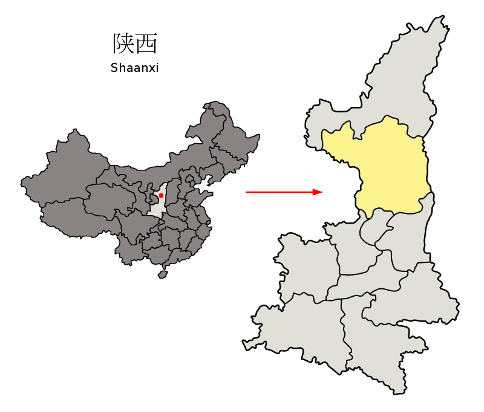
\includegraphics[width=0.6\textwidth]{figures/yanchang_map.png}
\caption{Location of Yanchang County in China}
\label{Figure: Yanchang}
\end{figure}

The apple farmers in Yanchang County predominantly cultivate late-maturing Fuji apples, which constitute approximately 85-90\% of the production. Some farmers also grow mid-maturing apples (5-10\%) and early-maturing apples (around 5\%). Farm-gate prices range from 2.5 to 12 yuan/kg and can be checked regularly. The yield per acre does not significantly differ among the three apple varieties.

Although there are over 260 villages in the county, the average number of fruit storage facilities is slightly over 100, meaning that there is less than one facility per administrative village. Cold storage facilities owned by apple growers in Yanchang County can be classified into two types: small-scale facilities capable of storing up to 50 tons and medium-sized facilities with a capacity of up to 500 tons. According to the government report, only 1.3\% of farmers possess their own small-scale cold storage facilities. However, many farmers rent cold storage facilities established by the township and large merchants. It is worth noting that the quality of fruit storage facilities constructed by township governments is subpar compared to those built by farmers themselves. Farmers contribute 60\% of the investment, while the government subsidizes the remaining 40\%.

Farmers in Yanchang County who do not adopt cold storage facilities have to sell their harvest within a month. On the other hand, farmers using cold storage facilities need to consider various factors and market conditions, including the time-varying competition among traders. With cold storage, they can market their produce until April or May of the following year without significant deterioration. Furthermore, they are not necessarily limited to selling to middlemen but also sometimes do retail selling to consumers directly, as storage facilities grant them temporal flexibility to find more potential buyers.

%------------------------------------------------------%
%------------------------------------------------------%
\subsection{Data}
\subsubsection{Sampling Procedure}
\noindent This study employs empirical tests using data collected from two rounds of a survey of 615 smallholder apple growers in Yanchang County, Central China, covering the 2024/2025 agricultural season. With Institutional Review Board (IRB) approval, the survey was conducted between October 10, 2024, and December 13, 2024. Given that the harvest season for Fuji apples in Central China concludes in mid-to-late October, followed immediately by the lean season, this period provides a relevant timeframe to analyze the evolving market conditions faced by farmers.

The survey was conducted in collaboration with the Yanchang-County Women's Federation (YWF), an organization responsible for public welfare and rural development in Yanchang County. In coordination with the Yanchang County Agricultural Bureau, the YWF facilitated access to micro-level data on apple growers, enabling a structured sampling approach. A one-layer stratified random sampling method was employed based on geographical location. Yanchang County consists of one urban subdistrict and seven rural towns. To ensure representativeness, the Yanchang County Agricultural Bureau determined the approximate sampling proportion for each town based on the number and density of fruit farmers (30\%:15\%:15\%:15\%:10\%:5\%:5\%:5\%). Following these proportions, smallholder apple-growing households were randomly selected from rosters provided by administrative villages within each town.

For the purpose of this study, smallholder apple growers are defined as farmers who cultivate no more than 50 mu of land and derive at least 90\% of their agricultural income from apple production. Additionally, to maintain sufficient sample sizes across towns, a minimum of 10 participating apple growers was ensured in each town, though no minimum was imposed at the village level.

The survey targeted farmers whose primary source of income is derived from growing red Fuji apples. The interviews were conducted with the household head, except in cases where the household head was elderly and no longer part of the active labor force. In such instances, the survey was conducted with the primary labor force member of the household.



%------------------------------------------------------%
\subsubsection{Measures of Farmers' Storage Usage and Procurement Competitiveness}
\noindent This study examines apple growers' cold storage usage and marketing timing decisions as key dependent variables. First, I define \texttt{Storage-Usage-Binary}, a binary indicator equal to 1 if a farmer used cold storage at harvest and 0 otherwise. Second, \texttt{Storage-Usage-Type} categorizes storage choices into four groups: \textit{Not\_use}, and three storage options—\textit{Rent\_large}, \textit{Rent\_small}, or \textit{Self\_built}—each indicating some form of cold storage usage. Third, \texttt{Time-to-Sell} measures the delay between harvest and sale, effectively representing storage duration. Sales occurring in October are classified as 1–4 weeks post-harvest, November as 5–8 weeks, and so forth, yielding interval-censored data with four predefined selling-time intervals: 1–4, 5–8, 9–12, and 13–28 weeks. Figure \ref{Figure: selling weeks distribution} illustrates the distribution of selling weeks by storage type.

\begin{figure}[H]
\centering
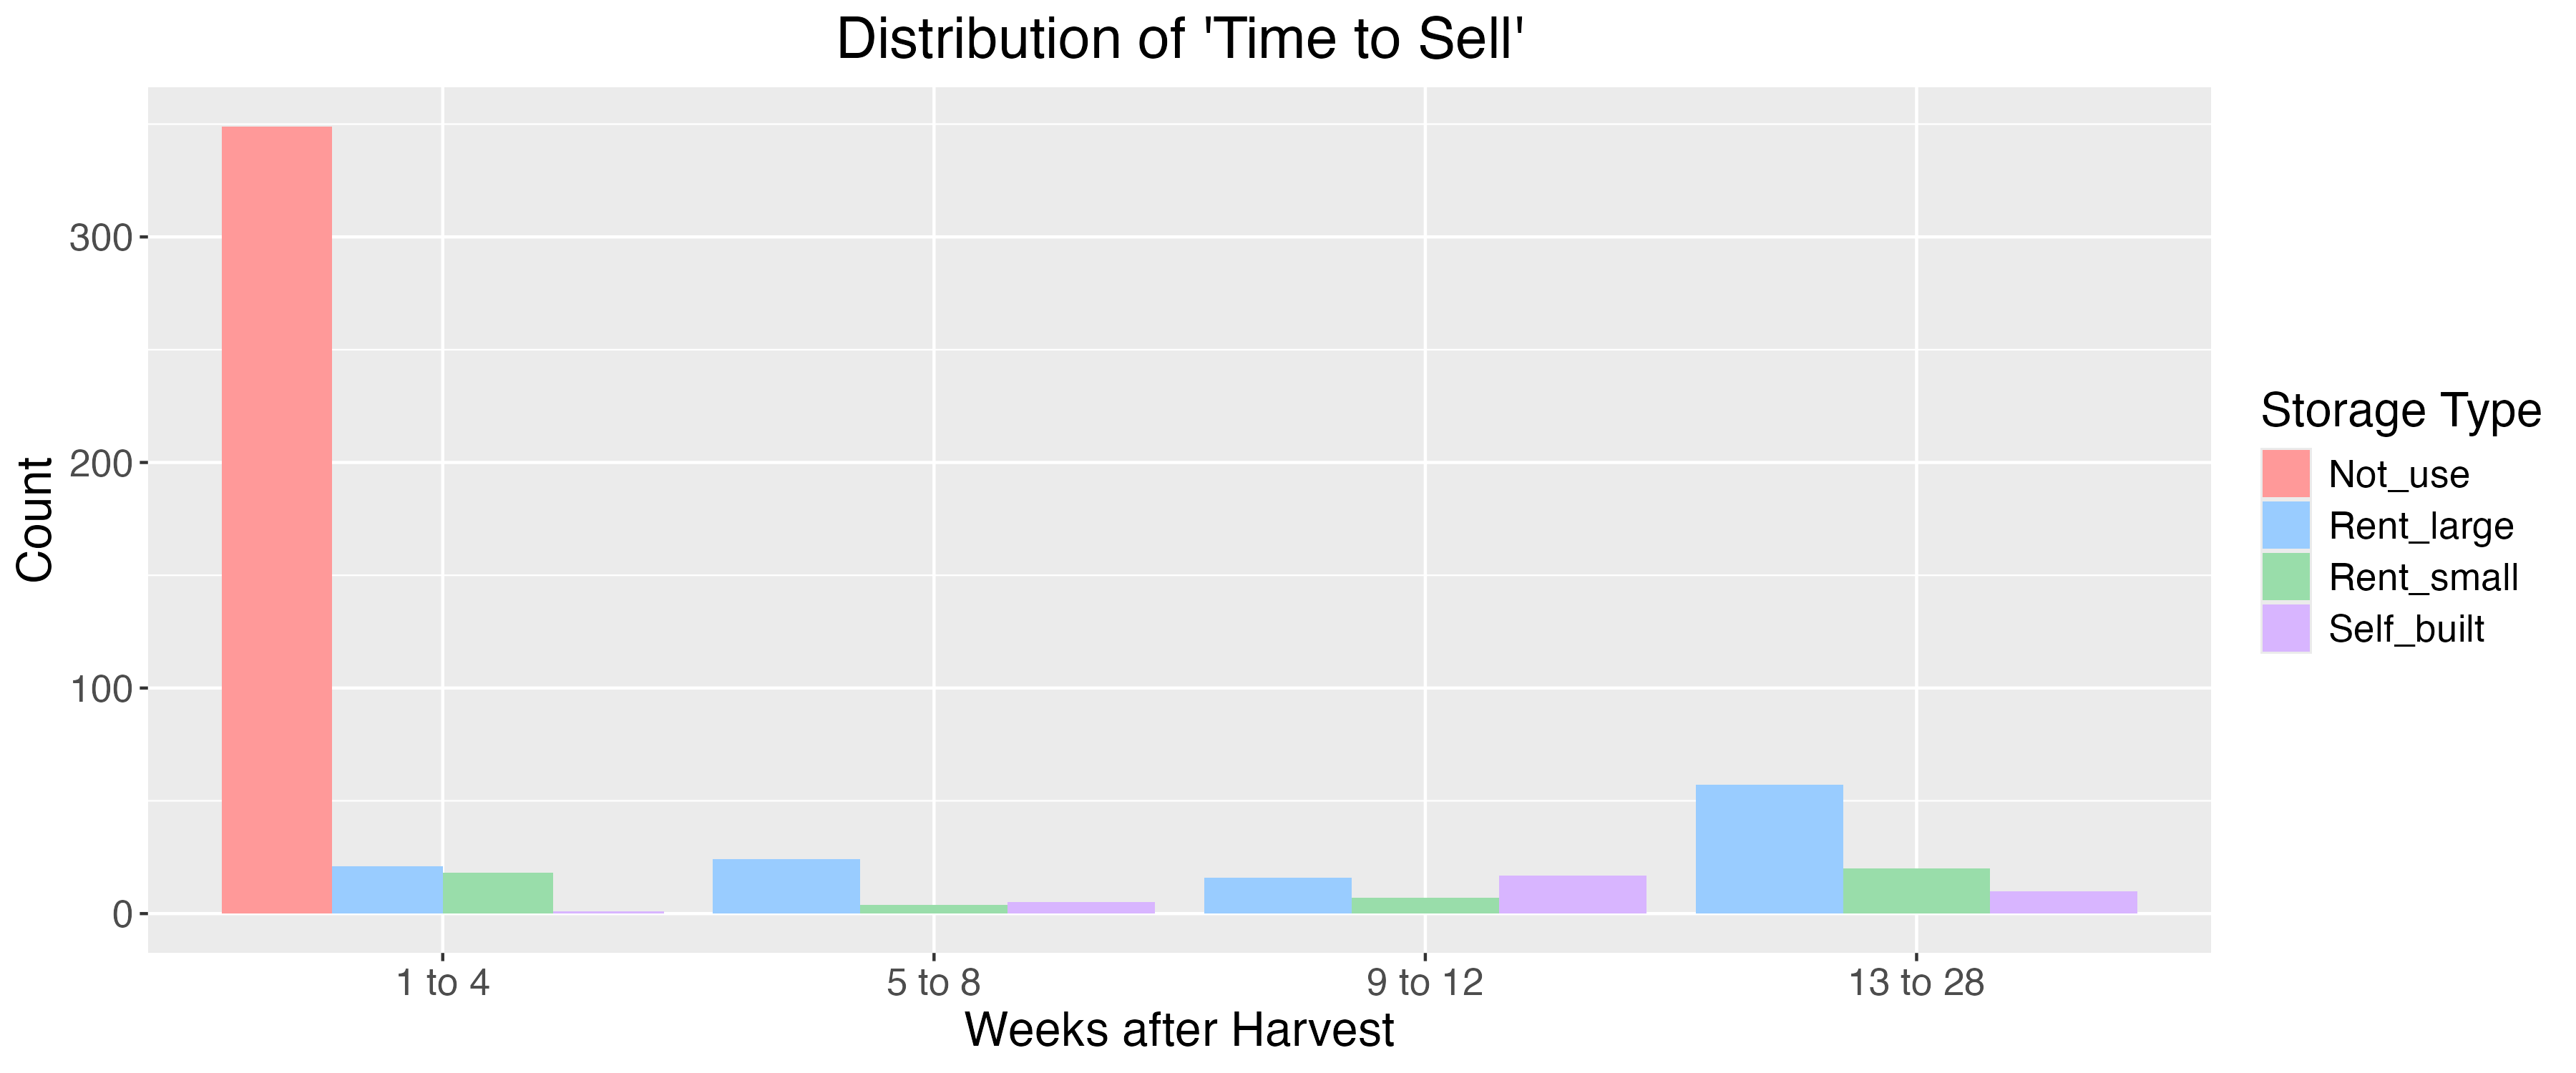
\includegraphics[width=1\textwidth]{figures/selling_weeks_distribution.png}
\caption{Distribution of Selling Weeks by Storage Type}
\label{Figure: selling weeks distribution}
\end{figure}

To capture inter-temporal variations in oligopsony power among buyers, farmers were asked to report:
\begin{enumerate}
    \item Their subjective assessment of buyer competition at harvest time (\texttt{Subjective buyer competitiveness}, measured on a 1–5 scale);
    \item Their expectations regarding changes in the number of traders over the subsequent three months (October 2024 onward), recorded as \texttt{Expect more buyers} and \texttt{Expect fewer buyers}.
\end{enumerate}

Additionally, the survey collected data on farmers' total annual agricultural income, production costs, storage expenses, and demographic characteristics to assess welfare implications.

To complement these farmer-level insights with market-level dynamics, a buyer survey was conducted in December 2024. This survey targeted 15 buyers, including the top five most influential local traders, and collected data on:
\begin{enumerate}
    \item The specific villages each buyer visited during the October harvest;
    \item The cold storage facilities from which they had procured apples over the preceding two months.
\end{enumerate}
These responses allow us to construct an objective measure of buyer concentration and inter-temporal competition. Inspired by \cite{macchiavello2021competition}, who used the number of mills within a 10 km radius as a competition metric, I define \texttt{Number of buyers} as the count of traders visiting each village post-harvest.


%------------------------------------------------------%
\subsubsection{Measure of Farmers' Risk Aversion and Liquidity Constraint}

Building on the methodology of \cite{jin2024losses}, whose fieldwork largely overlaps with mine, this study measures apple growers' risk preferences through two complementary approaches: a self-assessed risk preference scale and a behavioral measure based on a Holt-Laury-type lottery game. These methods provide both subjective and incentivized insights into farmers' risk attitudes, allowing for a more comprehensive understanding of their decision-making processes.

\paragraph{Self-Reported Risk Preference}
Following \cite{dohmen2011individual}, I assessed general risk attitudes by directly asking apple growers to rate their willingness to take risks on a scale from 1 to 5, where 1 represents \textit{``extreme risk aversion''} and 5 represents \textit{``very risk loving''}. While self-reported measures of risk tolerance are inherently subjective and may be influenced by social and peer effects, they serve as a useful supplementary indicator of perceived risk aversion. These perceptions likely influence farmers' broader economic decisions, including investment choices, production strategies, and financial risk management.

\paragraph{Holt-Laury-Type Lottery Game}
To complement the self-assessment, I implemented a behavioral measure using a modified Holt-Laury-type lottery game. Specifically, the survey asked apple growers how much they would be willing to pay for participation in a 50-50 lottery, where they had an equal chance of winning 200 CNY or receiving nothing. 

This approach is an adaptation of the \textit{multiple price list (MPL) choice task} from \cite{brick2012risk}, itself a variation of the widely used Holt-Laury risk elicitation method \cite{holt2002risk}. Participants were presented with various possible entry fees, ranging from 20 CNY to 120 CNY, and asked to decide whether they would pay each amount to enter the lottery. This effectively required them to choose between a \textit{``safe''} option (keeping their money) and a \textit{``risky''} option (participating in the lottery with an uncertain payoff). 

This design is particularly well-suited for field implementation, as it is straightforward and easy to understand for farmers with limited formal education. Additionally, it is practical for enumerators to administer and provides a more reliable measure of risk preferences by using real monetary stakes, which encourage truthful responses. Different willingness-to-pay (WTP) values for the lottery correspond to varying expected values and degrees of risk aversion, as depicted in Table \ref{tab:experiment_design}.

\begin{table}[H]
    \centering
    \footnotesize 
    \caption{Mini-brain Experiment Design: A Head-Tail Lottery Game}
    \renewcommand{\arraystretch}{1.2}
    \begin{tabular}{cccccc}
        \toprule
        \textbf{Option} & \textbf{Willingness to Pay} & \textbf{Outcome} & \textbf{EV$^{A}$--EV$^{B}$} & \textbf{CRRA Ranges} & \textbf{CRRA Adjusted}\\
        \midrule
        1 & 120 CNY & 200 CNY or 0 & 20 CNY & $-0.4 < r < 0$  & $r = -0.2$\\
        2 & 100 CNY & 200 CNY or 0 & 0 CNY & $0 < r < 0.2$  & $r= 0.1$ \\
        3 & 80 CNY & 200 CNY or 0 & -20 CNY & $0.2 < r < 0.4$  & $r= 0.3$ \\
        4 & 60 CNY & 200 CNY or 0 & -40 CNY & $0.4 < r < 0.6$  & $r= 0.5$ \\
        5 & 40 CNY & 200 CNY or 0 & -60 CNY & $0.6 < r < 0.7$  & $r=0.6$ \\
        6 & 20 CNY & 200 CNY or 0 & -80 CNY & $0.7 < r$  & $r= 0.9$ \\
        \bottomrule
    \end{tabular}
    \label{tab:experiment_design}
    \vspace{0.5em}
    \small Notes: EV = Expected Value. CRRA = Coefficient of Relative Risk Aversion.
\end{table}

\paragraph{Estimating Risk Aversion Using CRRA}
The switching point in this experiment—i.e., the highest price a participant is willing to pay for the lottery—provides insight into their risk attitude. Following \cite{chiappori2011relative}, who found that individuals generally exhibit constant relative risk aversion (CRRA), I assume a CRRA utility function of the form, $U(x) = \frac{x^{1-r}}{1 - r}$, where \(r\) represents the risk aversion coefficient. Under this specification, \(r > 0\) implies risk aversion, \(r = 0\) indicates risk neutrality, and \(r < 0\) reflects risk-seeking behavior.

Columns 5 and 6 in Table \ref{tab:experiment_design} present the implied CRRA ranges and the adjusted CRRA values used in the subsequent analysis. By examining these values, I can quantitatively assess the degree of risk aversion among apple growers, which is crucial for understanding their storage decisions and responses to market structural uncertainty.


%------------------------------------------------------%
\subsubsection{Descriptive Statistics}
\noindent The final dataset comprises 549 smallholder apple-growing households in Central China. Among them, 200 farmers used cold storage in the 2024–2025 agricultural year, with 33 storing apples in self-built facilities, 49 using small-scale commercial storage, and 118 opting for large-scale commercial storage. Figure \ref{Figure: pie and radar chart} presents the distribution of storage usage types and the sources of their price information. 

\begin{figure}[htp]
\centering
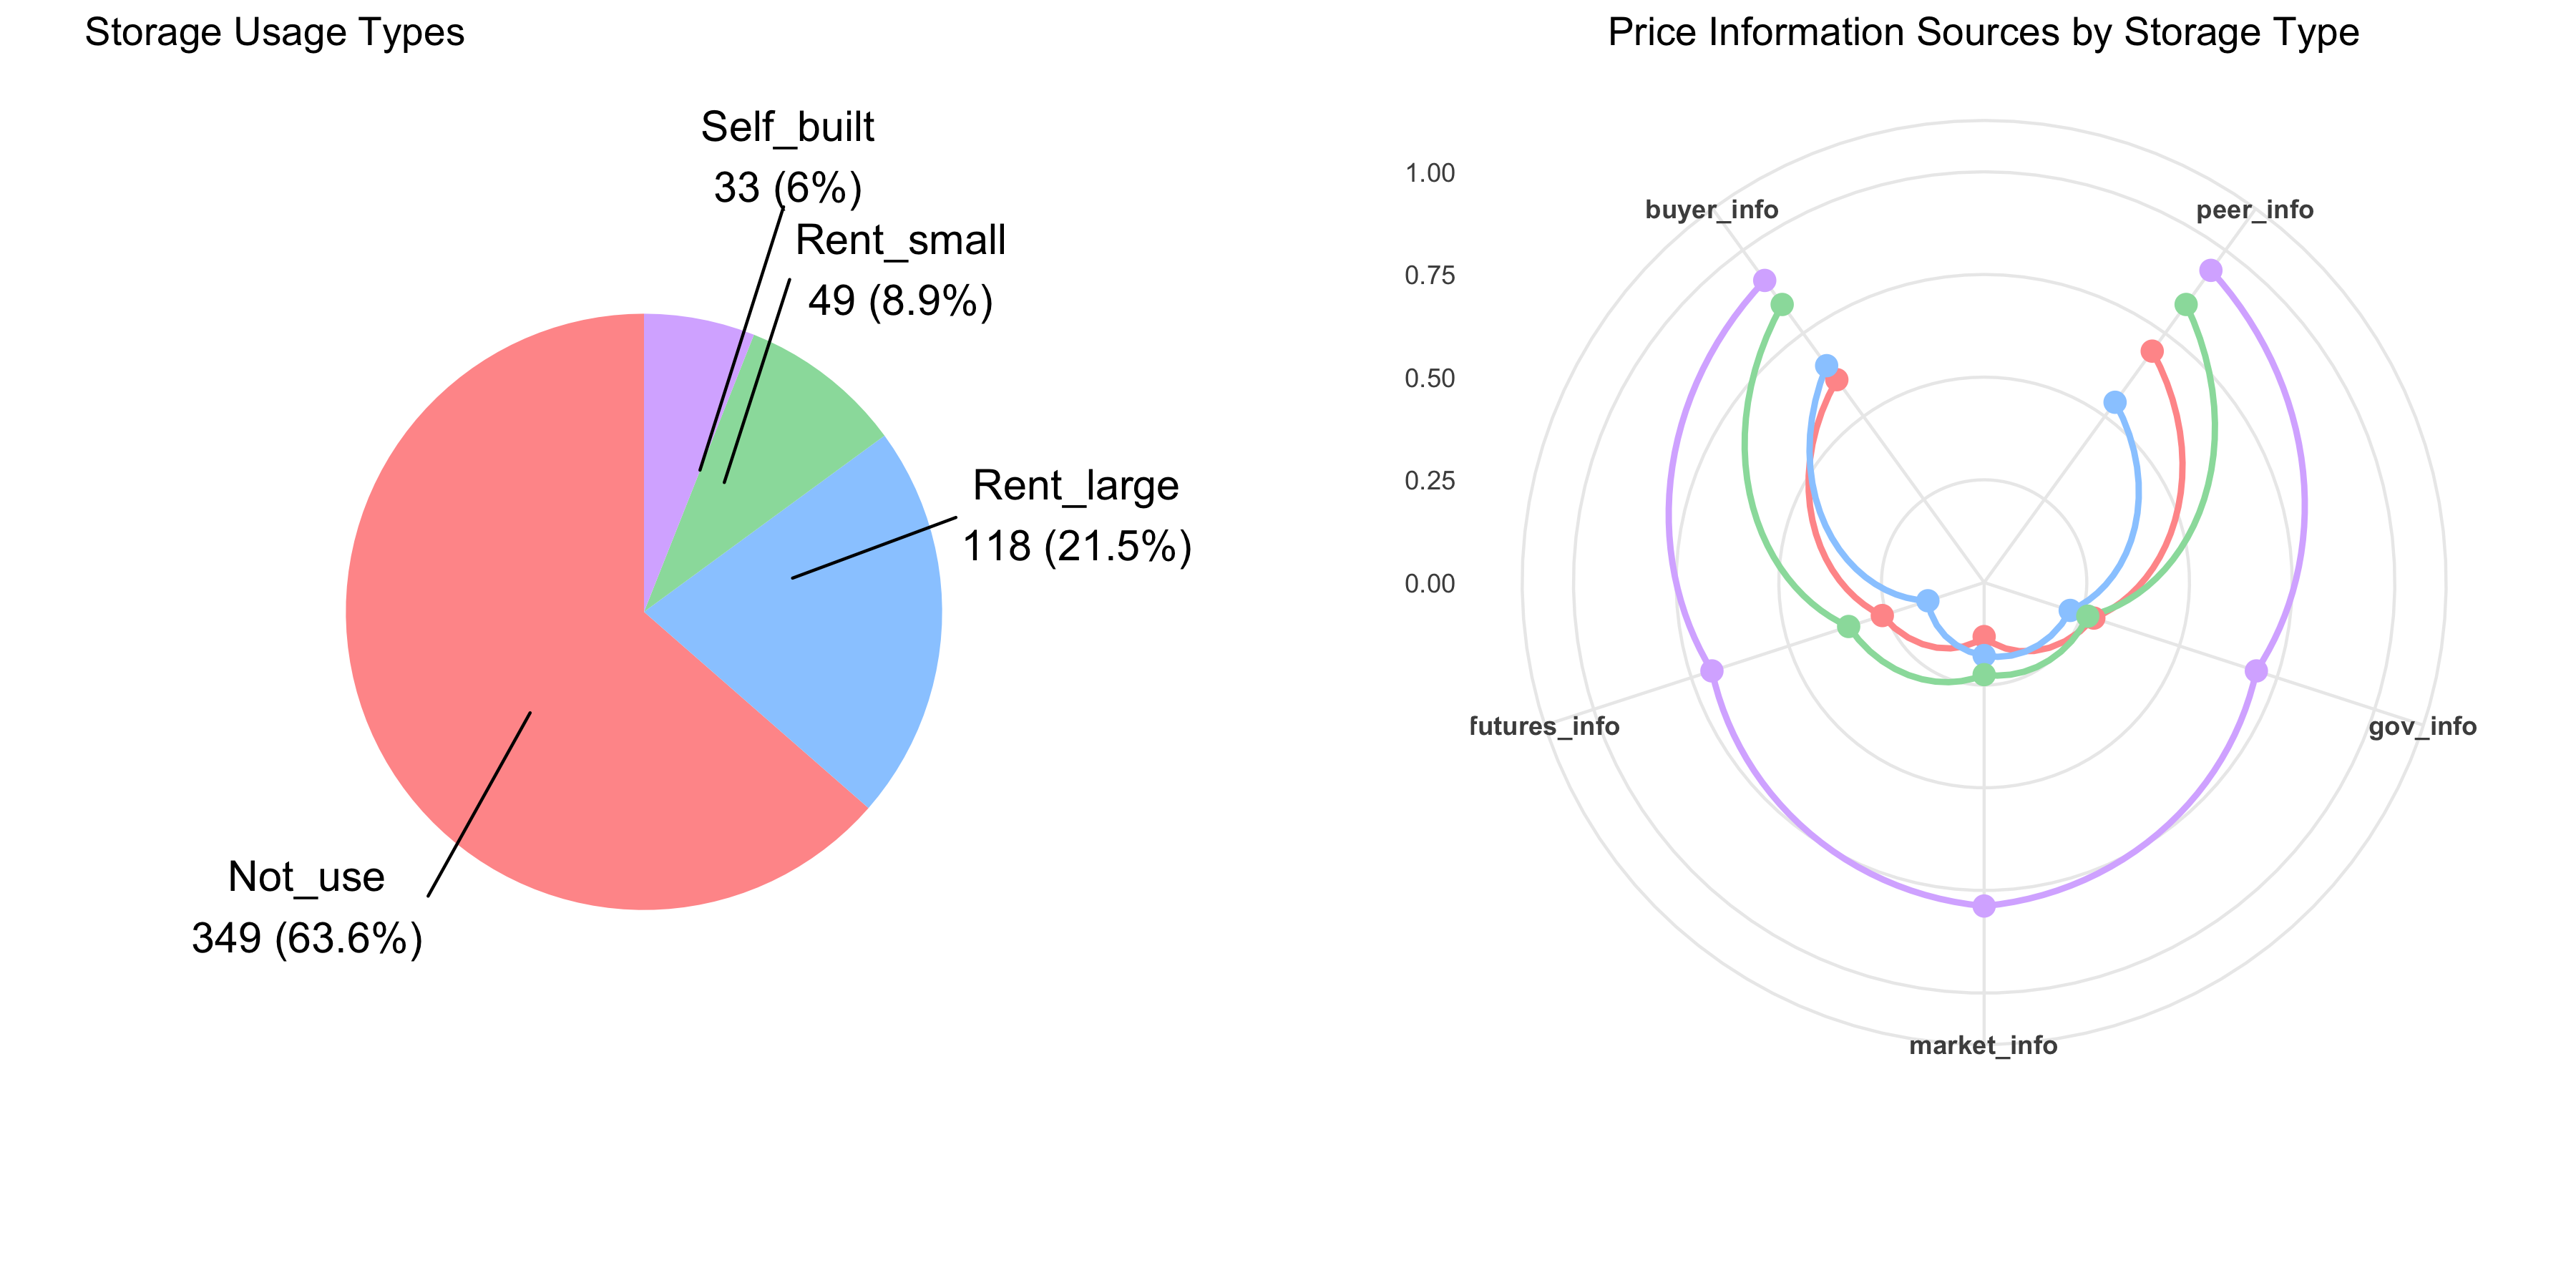
\includegraphics[width=1\textwidth]{figures/storage_usage_analysis_soft_colors.png}
\caption{Distribution of Storage Usage Types and Their Price Information Sources}
\label{Figure: pie and radar chart}
\end{figure}

These 200 storage users constitute a key sub-sample for analyzing storage behavior. Table \ref{tab: summary statistics} presents summary statistics for both the full sample and this sub-sample, covering key variables such as \texttt{Number of buyers} at harvest, \texttt{Subjective buyer competitiveness}, and farmers' expectations of future buyer competition (Panel E), along with other survey variables used in this study. The data confirms that the sample consists of smallholder apple-growing households, with an average landholding of just 2.05 acres and an average yield of 11.46 tons. On average, households comprise 2 to 3 members, with fewer than two active laborers supporting livelihoods at a mean age of 59.08. Their total annual income is under ten thousand USD (69,237.85 RMB = 9,540 USD), with more than 90\% derived from apple cultivation. A detailed description of each variable is provided in the appendix.

\begin{figure}[htp]
\centering
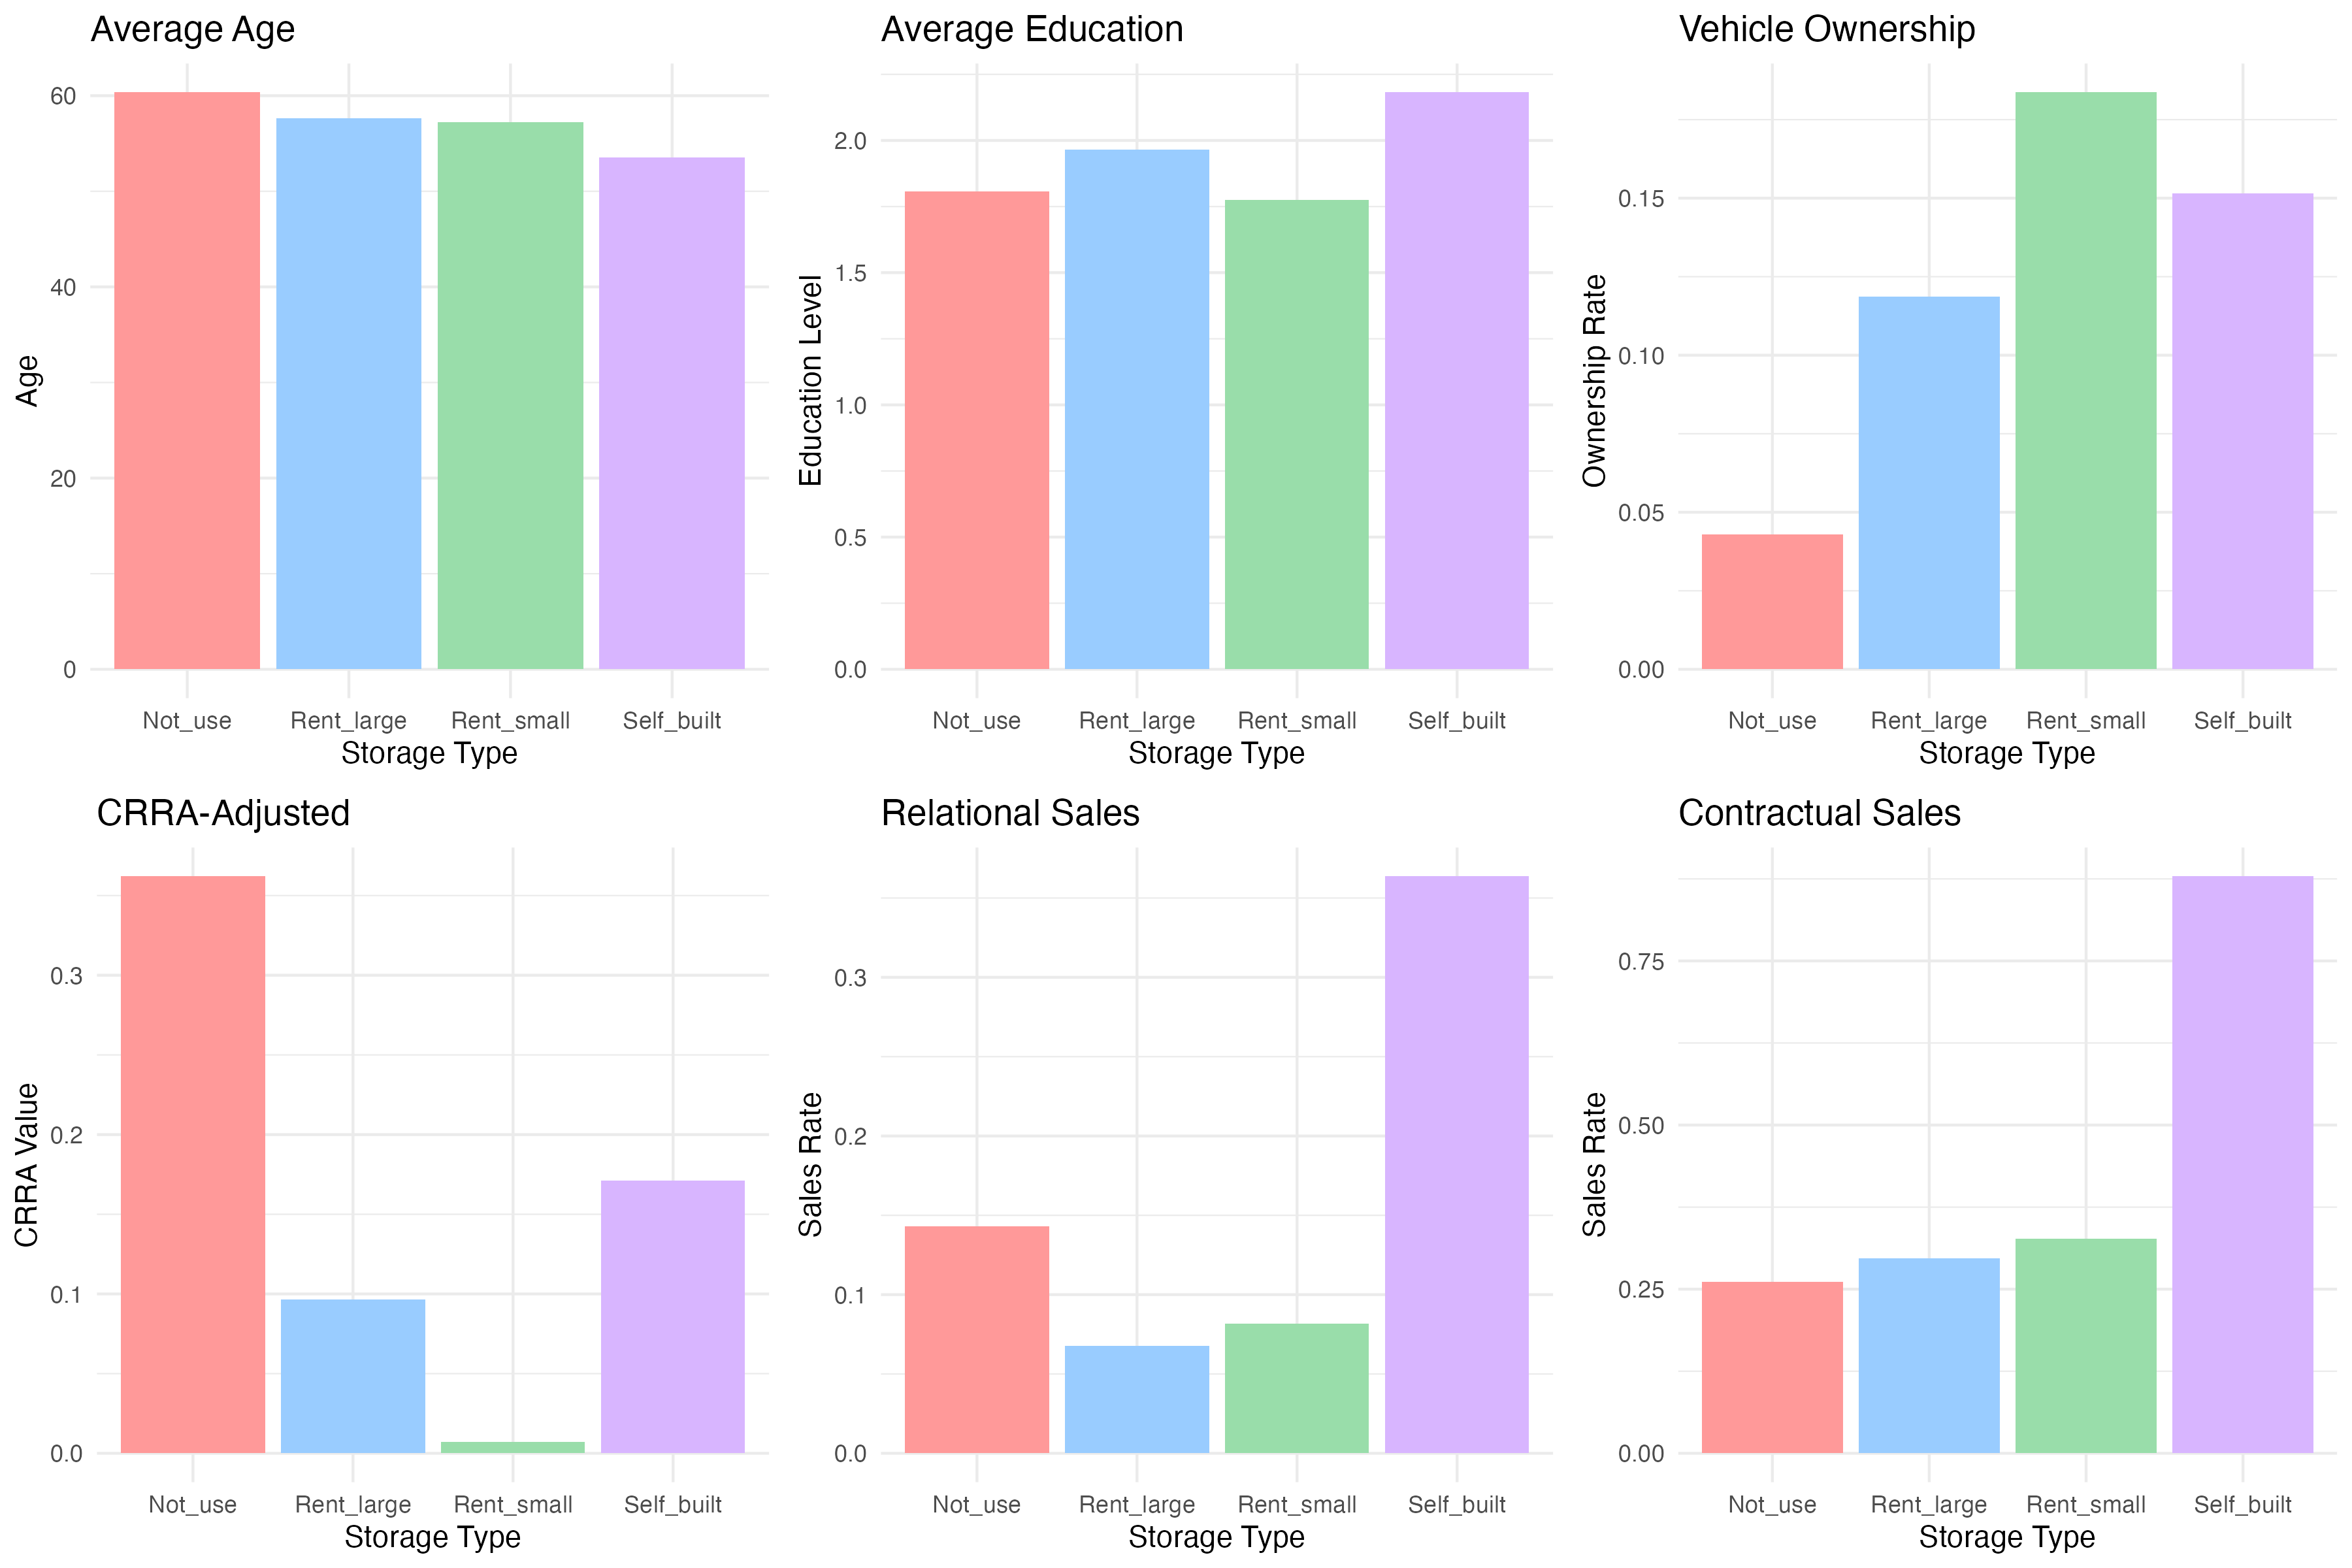
\includegraphics[width=1\textwidth]{figures/combined_storage_metrics.png}
\caption{Demographics by Storage Type}
\label{Figure: Demographics by Storage Type}
\end{figure}

Figure \ref{Figure: Demographics by Storage Type} presents a cross-group comparison of six key demographics: age, education level, car/truck ownership, risk aversion (adjusted CRRA), and participation in relational and implicit contractual sales. While the patterns within storage users are not entirely clear, a comparison between storage users (blue, green, and purple) and non-users (red) reveals several distinctions. Storage users tend to be slightly younger, more educated, less risk-averse, and more likely to own vehicles. Notably, farmers who use self-built cold storage stand out in their engagement with relational and contractual sales.


\begin{table}[H]
\centering
\caption{Summary Statistics by Storage Usage}
\label{tab: summary statistics}
\resizebox{\textwidth}{!}{%
\begin{tabular}{lccccc}
\toprule
 & \multicolumn{2}{c}{Storage Users} & \multicolumn{2}{c}{Non-Users} & Difference \\
\cmidrule(lr){2-3} \cmidrule(lr){4-5}
Variable & Mean & SD & Mean & SD & t-statistic \\
\midrule
\multicolumn{6}{l}{\textbf{Panel A: Farmer Demographics}} \\
Age (years) & 56.87 & (9.57) & 60.35 & (9.63) & -4.09*** \\
Household size (persons) & 2.71 & (1.21) & 2.58 & (1.10) & 1.24 \\
Labor size (persons) & 1.74 & (0.71) & 1.60 & (0.66) & 2.20** \\
Highest education (level) & 1.96 & (0.67) & 1.81 & (0.76) & 2.35** \\
Family ever village leader (0/1) & 0.24 & (0.43) & 0.06 & (0.24) & 5.37*** \\
Liquidity constrained (0/1) & 0.15 & (0.36) & 0.16 & (0.37) & -0.17 \\
\addlinespace
\multicolumn{6}{l}{\textbf{Panel B: Production and Consumption}} \\
Apple yield (tons) & 11.08 & (7.56) & 11.68 & (14.12) & -0.64 \\
Land size (acre) & 2.60 & (1.70) & 1.72 & (0.99) & 6.69*** \\
Bad apple ratio & 2.31 & (1.20) & 2.02 & (1.18) & 2.78*** \\
Apple income (USD) & 10127.22 & (6108) & 8289 & (6465) & 3.32*** \\
Total income (USD) & 10919 & (6445) & 8990 & (7334) & 3.21*** \\
Labor cost (USD) & 1911 & (1593) & 1343 & (1258) & 4.33*** \\
Family consumption (USD) & 7117 & (8899) & 5059 & (3869) & 3.11*** \\
\addlinespace
\multicolumn{6}{l}{\textbf{Panel C: Storage and Risk-Related Factors}} \\
Car/truck ownership (0/1) & 0.14 & (0.35) & 0.04 & (0.20) & 3.61*** \\
Natural disaster insurance (0/1) & 0.35 & (0.48) & 0.33 & (0.47) & 0.49 \\
Price insurance (0/1) & 0.62 & (0.49) & 0.65 & (0.48) & -0.78 \\
CRRA adjusted (coef) & 0.09 & (0.37) & 0.36 & (0.45) & -7.75*** \\
Storage in village (0/1) & 0.38 & (0.49) & 0.20 & (0.60) & 3.74*** \\
Far to small storage (0/1) & 0.52 & (0.50) & 0.79 & (0.41) & -6.71*** \\
Far to large storage (0/1) & 0.89 & (0.32) & 0.91 & (0.28) & -1.07 \\
Storage for wider marketing (0/1) & 0.88 & (0.33) & 0.30 & (0.46) & 16.90*** \\
Storage as bargaining tool (0/1) & 0.80 & (0.40) & 0.29 & (0.46) & 13.79*** \\
\addlinespace
\multicolumn{6}{l}{\textbf{Panel D: Marketing}} \\
Highest price per pound (USD/lb) & 0.41 & (0.09) & 0.38 & (0.10) & 3.94*** \\
Good price per pound (USD/lb) & 0.40 & (0.08) & 0.37 & (0.10) & 3.29*** \\
WeChat selling (0/1) & 0.15 & (0.36) & 0.00 & (0.00) & 6.04*** \\
Relational selling (0/1) & 0.12 & (0.33) & 0.14 & (0.35) & -0.78 \\
Contract selling (0/1) & 0.40 & (0.49) & 0.26 & (0.44) & 3.32*** \\
\addlinespace
\multicolumn{6}{l}{\textbf{Panel E: Market Competitive Conditions}} \\
Expect more buyers (0/1) & 0.46 & (0.50) & 0.06 & (0.23) & 10.75*** \\
Expect fewer buyers (0/1) & 0.16 & (0.39) & 0.19 & (0.39) & -0.90 \\
Number of buyers at harvest (count) & 3.83 & (2.45) & 3.12 & (1.91) & 3.51*** \\
Subjective buyer competitiveness (1/5) & 2.92 & (0.84) & 3.06 & (0.69) & -2.08** \\
\hline
\hline
Observations & 200 & & 349 & & 549 \\
\bottomrule
\end{tabular}% 
} % End of resizebox 
\begin{tablenotes} 
\item \textit{Notes:} The table presents means and standard deviations (in parentheses) for each variable by group. T-statistics from two-sample t-tests are reported to indicate statistical significance of differences between groups. Significance levels are denoted by asterisks: * p$<$0.1, ** p$<$0.05, *** p$<$0.01. In addition, monetary values have been converted from Chinese Yuan (RMB) to US Dollars (USD), land area from mu to acres, and apple prices from RMB/kg to USD/pound using appropriate conversion rates. 
\end{tablenotes} 
\end{table}


In Table \ref{tab: summary statistics}, the average highest price offers received by farmers in the full sample is \$0.38 per pound (6.12 RMB/kg), while the average transaction price is \$0.37 per pound (5.96 RMB/kg), both of which are slightly higher for storage users. As shown in Figure \ref{Figure: selling price bubble}, apple growers without cold storage are constrained to selling at harvest (October), with transaction prices exhibiting a wide range that narrows over time. Prices tend to rise in November and December, though transaction volumes decline. Storage users who sell later may achieve higher prices, reaching \$0.50–\$0.60 per pound in December. This suggests a potential trade-off between immediate liquidity and potential price gains through storage, depending on market conditions.

\begin{figure}[H]
\centering
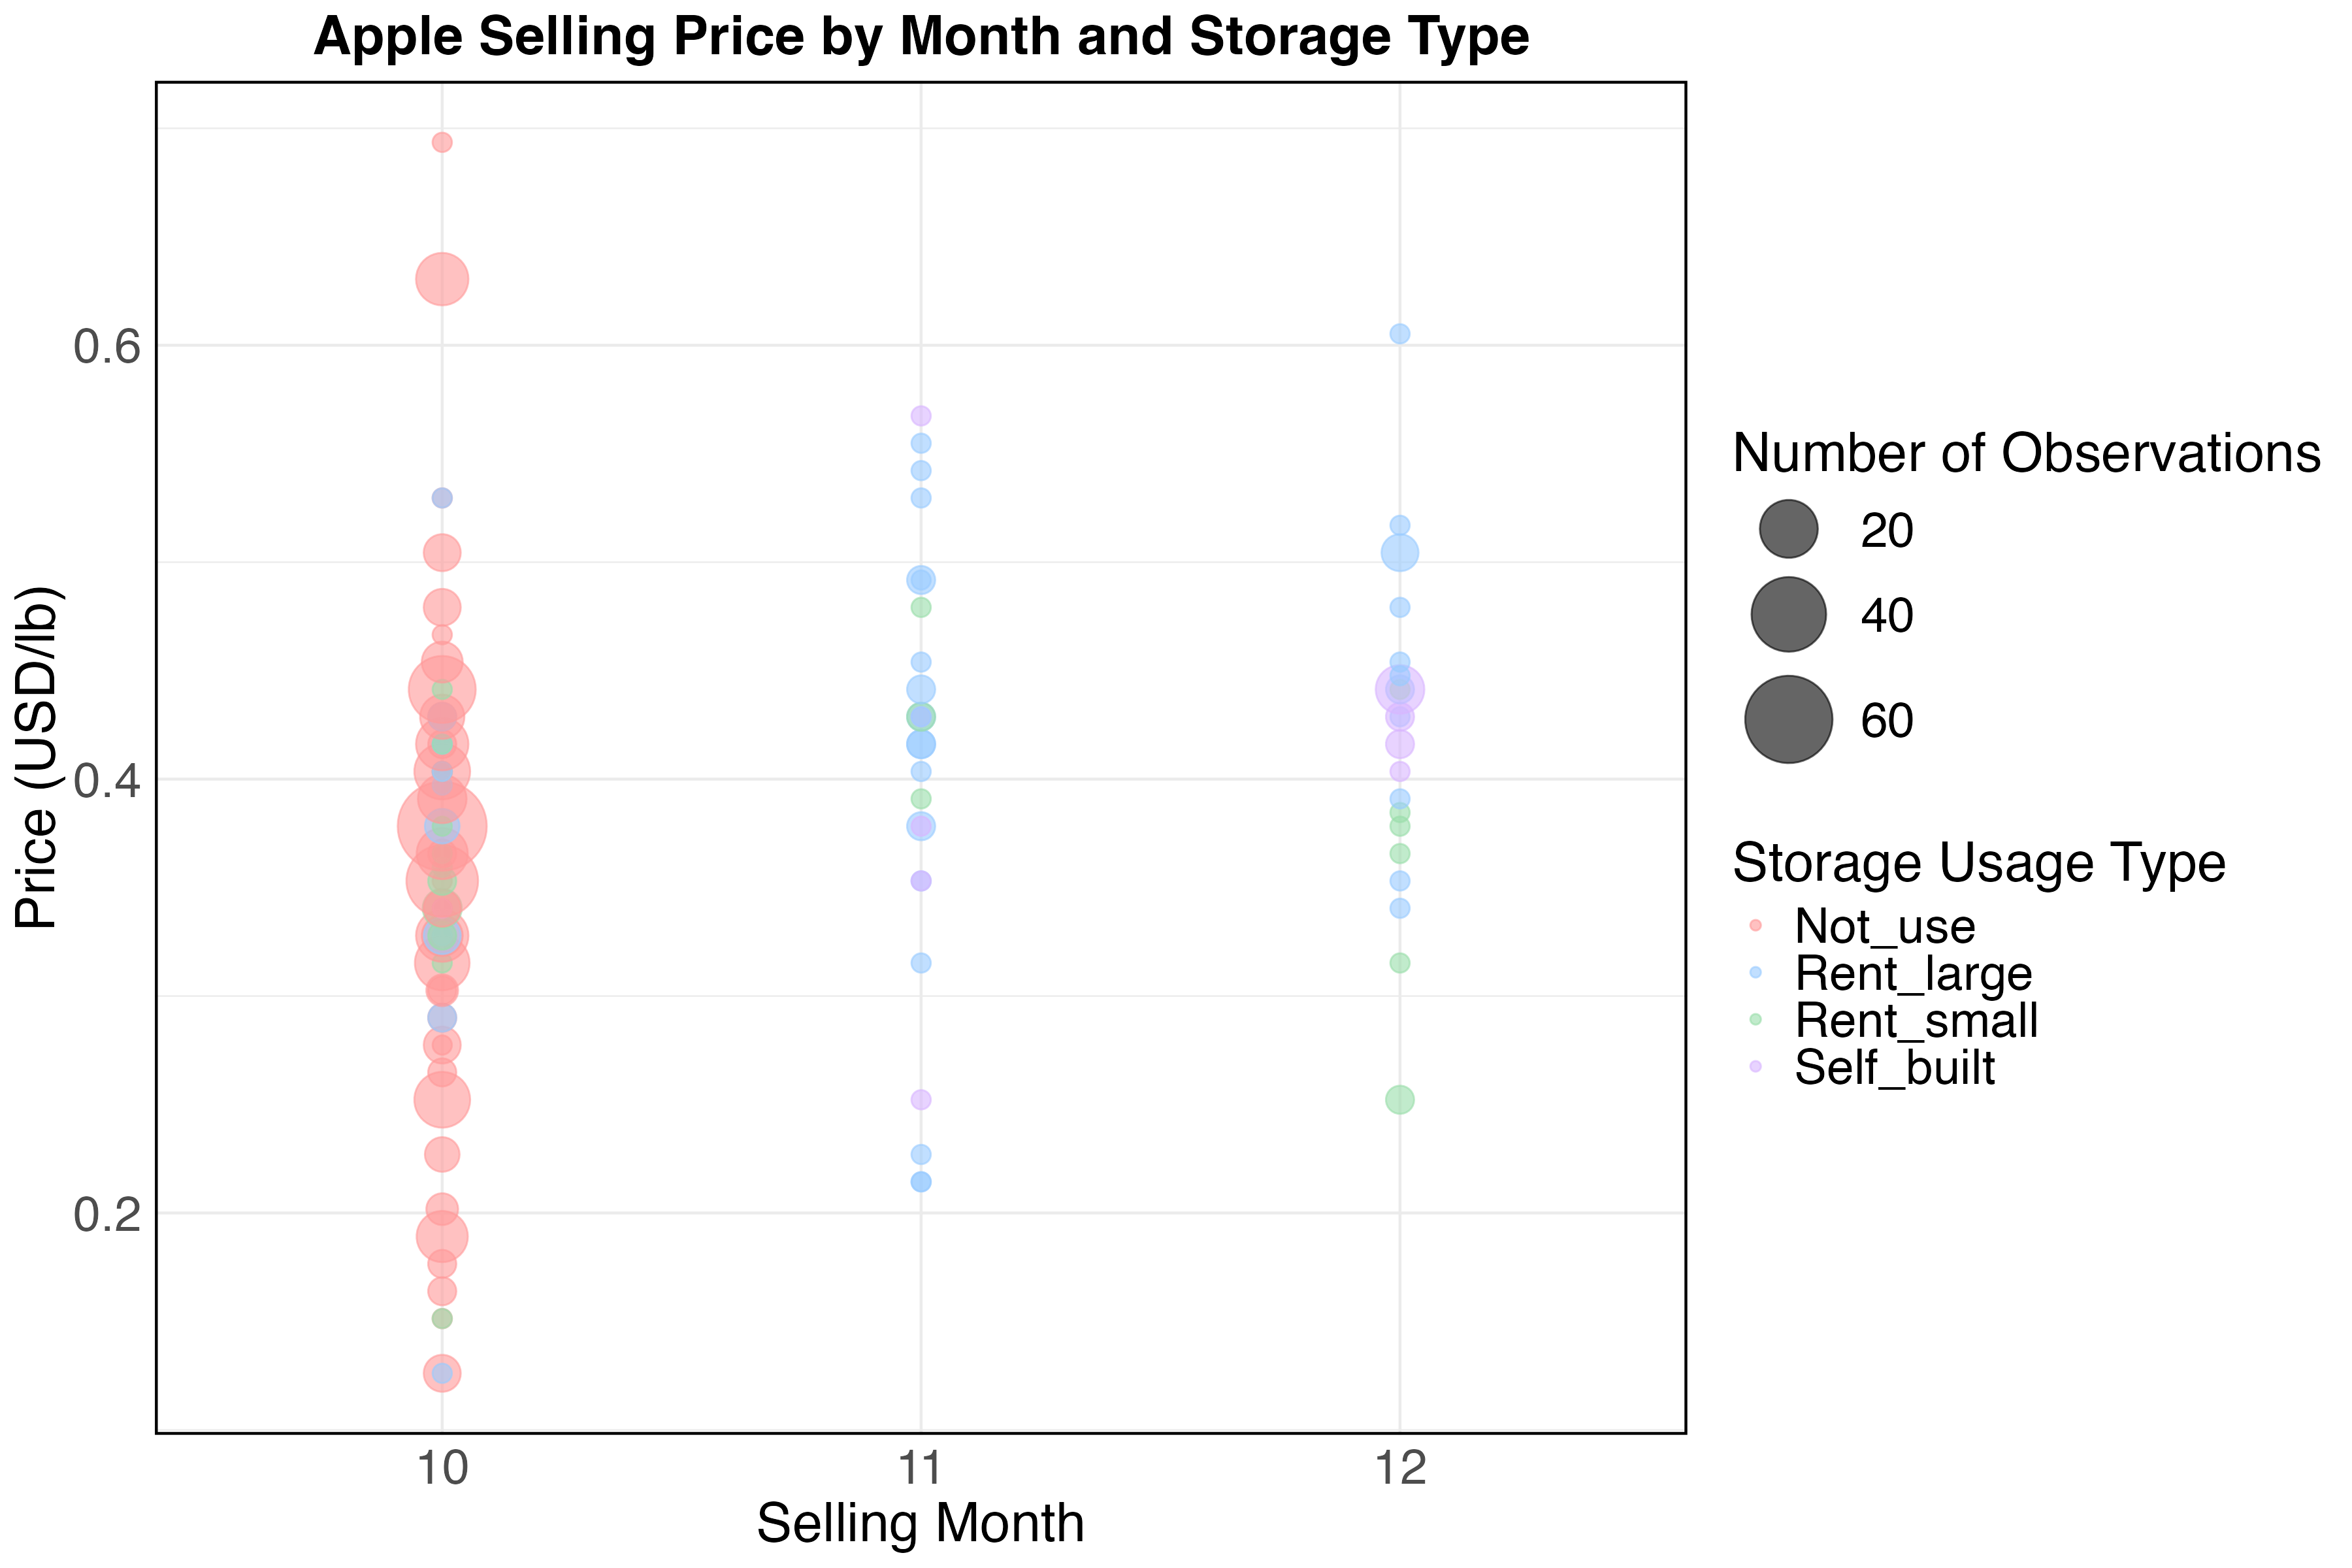
\includegraphics[width=1\textwidth]{figures/apple_price_bubble_plot.png}
\caption{Apple Selling Price by Month and Storage Type}
\label{Figure: selling price bubble}
\end{figure}

However, without post hoc knowledge or due to negative past experiences, most farmers in my sample chose not to store their produce. Table \ref{tab:non_storage_reasons} summarizes the reasons why farmers choose not to use storage facilities. Among the 349 non-storage farmers, the most common reason is the belief that they cannot sell at higher prices later, cited by 60.75\% of respondents. Additionally, 28.65\% of farmers perceive storage as too risky, while 22.92\% find the associated costs prohibitive. A smaller proportion, 8.02\%, report that their produce has been pre-ordered, eliminating the need for storage.

\begin{table}[H]
    \centering
    \footnotesize
    \caption{Reasons for Not Using Storage Facilities}
    \label{tab:non_storage_reasons}
    \resizebox{\textwidth}{!}{%
        \begin{tabular}{lcccc}
            \toprule
            \textbf{Reason} & High Storage Costs & Pre-ordered Produce & Cannot Sell High Later & Too Risky \\
            \midrule
            \textbf{Percentage} & 22.92\% & 8.02\% & 60.75\% & 28.65\% \\
            \bottomrule
        \end{tabular}%
        }
        \begin{tablenotes}
            \item \textit{Notes:} This table presents the reasons provided by the 349 farmers who do not use storage facilities, expressed as percentages of total non-storage farmers.
        \end{tablenotes}
\end{table}


%------------------------------------------------------%
%------------------------------------------------------%
\newpage
\subsection{Empirical Specification}

\subsubsection{Buyers' Competitiveness at Harvest and Storage Decisions}
This section presents the results of a logistic regression model with town-level fixed effects examining the determinants of binary storage usage. The dependent variable is whether an individual engages in storage ($S_i = 1$) or not ($S_i = 0$). The key independent variables fall into two categories: (1) subjective beliefs about buyer competition at harvest ($B^s_i$), measured on a scale from 1 to 5, where higher values indicate stronger perceived competition, and (2) the objective number of buyers at harvest ($B^o_i$), representing the actual market structure farmers face. The estimated logit model with town-level fixed effects is specified as follows:
\begin{equation}
\text{logit} \left( P(S_i = 1) \right) = \beta_0 + \beta_1 B^o_i + \beta_2 B^s_i + \beta_3 X_i + \beta_4 (B^o_i \times B^s_i) + \gamma_t + \varepsilon_i
\end{equation}
where $X_i$ represents a vector of control variables including demographic and risk-related factors, $\gamma_t$ denotes town-level fixed effects, and $\varepsilon_i$ is the error term.


% Table created by stargazer v.5.2.3 by Marek Hlavac, Social Policy Institute. E-mail: marek.hlavac at gmail.com
% Date and time: Wed, Sep 24, 2025 - 19:45:19
\begin{table}[H] \centering 
  \caption{Logistic Regression Results} 
  \label{tab: binary storage ~ buyers' competition at harvest} 
\footnotesize 
\begin{tabular}{@{\extracolsep{5pt}}lccc} 
\\[-1.8ex]\hline 
\hline \\[-1.8ex] 
 & \multicolumn{3}{c}{\textit{Dependent variable:}} \\ 
\cline{2-4} 
\\[-1.8ex] & \multicolumn{3}{c}{Storage Usage (Binary)} \\ 
 & Model 1 & Model 2 & Model 3 \\ 
\\[-1.8ex] & (1) & (2) & (3)\\ 
\hline \\[-1.8ex] 
 Number of Buyers & 0.004 &  & 0.45$^{***}$ \\ 
  & (0.05) &  & (0.10) \\ 
  & & & \\ 
 Subjective Belief &  & $-$0.52$^{***}$ & $-$1.55$^{***}$ \\ 
  &  & (0.16) & (0.28) \\ 
  & & & \\ 
 Age & $-$0.03$^{**}$ & $-$0.03$^{**}$ & $-$0.02$^{*}$ \\ 
  & (0.01) & (0.01) & (0.01) \\ 
  & & & \\ 
 Education Level & 0.38$^{**}$ & 0.36$^{**}$ & 0.31$^{*}$ \\ 
  & (0.17) & (0.17) & (0.18) \\ 
  & & & \\ 
 Family Village Leader & 1.26$^{***}$ & 1.23$^{***}$ & 1.17$^{***}$ \\ 
  & (0.35) & (0.35) & (0.36) \\ 
  & & & \\ 
 CRRA Adjusted & $-$1.08$^{***}$ & $-$0.96$^{***}$ & $-$0.99$^{***}$ \\ 
  & (0.29) & (0.29) & (0.30) \\ 
  & & & \\ 
 Liquidity Constrained & 0.05 & $-$0.05 & $-$0.03 \\ 
  & (0.31) & (0.32) & (0.33) \\ 
  & & & \\ 
 Constant & $-$0.80 & 0.86 & 2.37$^{*}$ \\ 
  & (1.06) & (1.18) & (1.21) \\ 
  & & & \\ 
\hline \\[-1.8ex] 
Town Fixed Effects & Yes & Yes & Yes \\ 
Observations & 549 & 549 & 549 \\ 
Log Likelihood & $-$237.94 & $-$232.29 & $-$221.10 \\ 
Akaike Inf. Crit. & 491.88 & 480.58 & 460.20 \\ 
Bayesian Inf. Crit. & 526.34 & 515.04 & 498.97 \\ 
\hline 
\hline \\[-1.8ex] 
\textit{Note:}  & \multicolumn{3}{r}{$^{*}$p$<$0.1; $^{**}$p$<$0.05; $^{***}$p$<$0.01} \\ 
\end{tabular} 
\end{table} 


The primary interest here is the effect of farmers' subjective beliefs regarding buyers' competition at harvest on storage decisions. This measure ranges from 1 to 5, where a higher value indicates a stronger belief in intense competition among buyers. The results indicate a strong and statistically significant negative effect of subjective beliefs on storage usage across all models where they are included. Specifically, in Model 2, the coefficient is -0.52 (p $<$ 0.01), increasing in magnitude to -1.55 in Model 3 and -2.60 in Model 4 (both p $<$ 0.01). This suggests that as farmers perceive higher competition among buyers, they are significantly less likely to engage in storage. The strengthening effect in later models, which control for additional interactions, underscores the robustness of this finding.

On the other hand, the actual number of buyers present at harvest appears to have little to no impact on farmers' storage behavior. In Model 1, the coefficient is 0.003 and statistically insignificant, while in Models 3 and 4, the coefficients (0.45 and -0.39, respectively) suggest inconsistent effects. This weak and erratic relationship indicates that farmers’ storage decisions are shaped more by their subjective perceptions of market conditions rather than the objective number of buyers operating in the market.

At first glance, the negligible effect of the actual number of traders may seem surprising, as it implies that the degree of buyer competition at harvest—at least as measured by the count of buyers—has little influence on storage decisions. Intuitively, one might expect that more buyers would lead to greater competition, higher prices, and, consequently, increased incentives for farmers to store their produce in anticipation of favorable selling conditions. However, the findings suggest otherwise, which raises important questions about the underlying market structure and the reliability of buyer count as a proxy for competition.

One key explanation for this discrepancy lies in the existence of buyer collusion, as discussed in the first chapter. If buyers collude—either explicitly or implicitly—to coordinate prices, then an increase in the number of buyers does not necessarily translate into increased competition. This is especially relevant in markets where many buyers act as intermediaries or agents for larger firms. In such cases, these agents may have limited autonomy in setting prices and may simply adhere to predetermined price offers dictated by their parent firms. When collusion among these agents is near perfect, the number of buyers ceases to be a meaningful indicator of actual market competitiveness.

This dynamic likely shapes farmers' perceptions. If farmers are aware that many traders operate under the influence of a few dominant firms, they may not view the mere presence of more buyers as an assurance of greater competition. Instead, their beliefs about competition may be shaped by informal market signals, previous experiences, and interactions with traders. For example, if farmers observe that prices remain relatively stable despite fluctuations in the number of buyers, they may conclude that true competition is lacking. Consequently, their storage decisions align more closely with their perception of competitive intensity rather than the raw count of buyers. This reasoning underscores the limitations of using the number of buyers as a standalone metric for market competition. In contexts where buyer collusion is prevalent, farmers may rationally discount the relevance of this measure in their decision-making process. Instead, they may rely on subjective assessments that better capture the market dynamics they actually face.

Furthermore, it is worth noting that the interaction effect between the number of buyers and farmers' subjective beliefs about buyer competition at harvest in the logistic model cannot be directly interpreted from the coefficient ($\beta = 0.25$, $p < 0.01$). A direct interpretation may misleadingly suggest that the two variables offset each other. Following \cite{ai2003interaction}, I calculate the correct interaction effect as the cross-partial derivative of the predicted probability with respect to both variables: $$\frac{\partial^2 P}{\partial x_1 \partial x_2} = \beta_{12} \cdot f(z) + \bigl(\beta_1 + \beta_{12} \, x_2\bigr) \cdot \bigl(\beta_2 + \beta_{12} \, x_1\bigr) \cdot f(z) \cdot \Bigl(1 - 2F(z)\Bigr)$$ This analysis reveals that the interaction effect varies substantially across observations, ranging from negative to positive values depending on farmers' characteristics. The magnitude and statistical significance of the effect also vary with the predicted probability of storage usage, as illustrated in Figure \ref{Figure: interaction effects}.

\begin{figure}[ht]
\centering
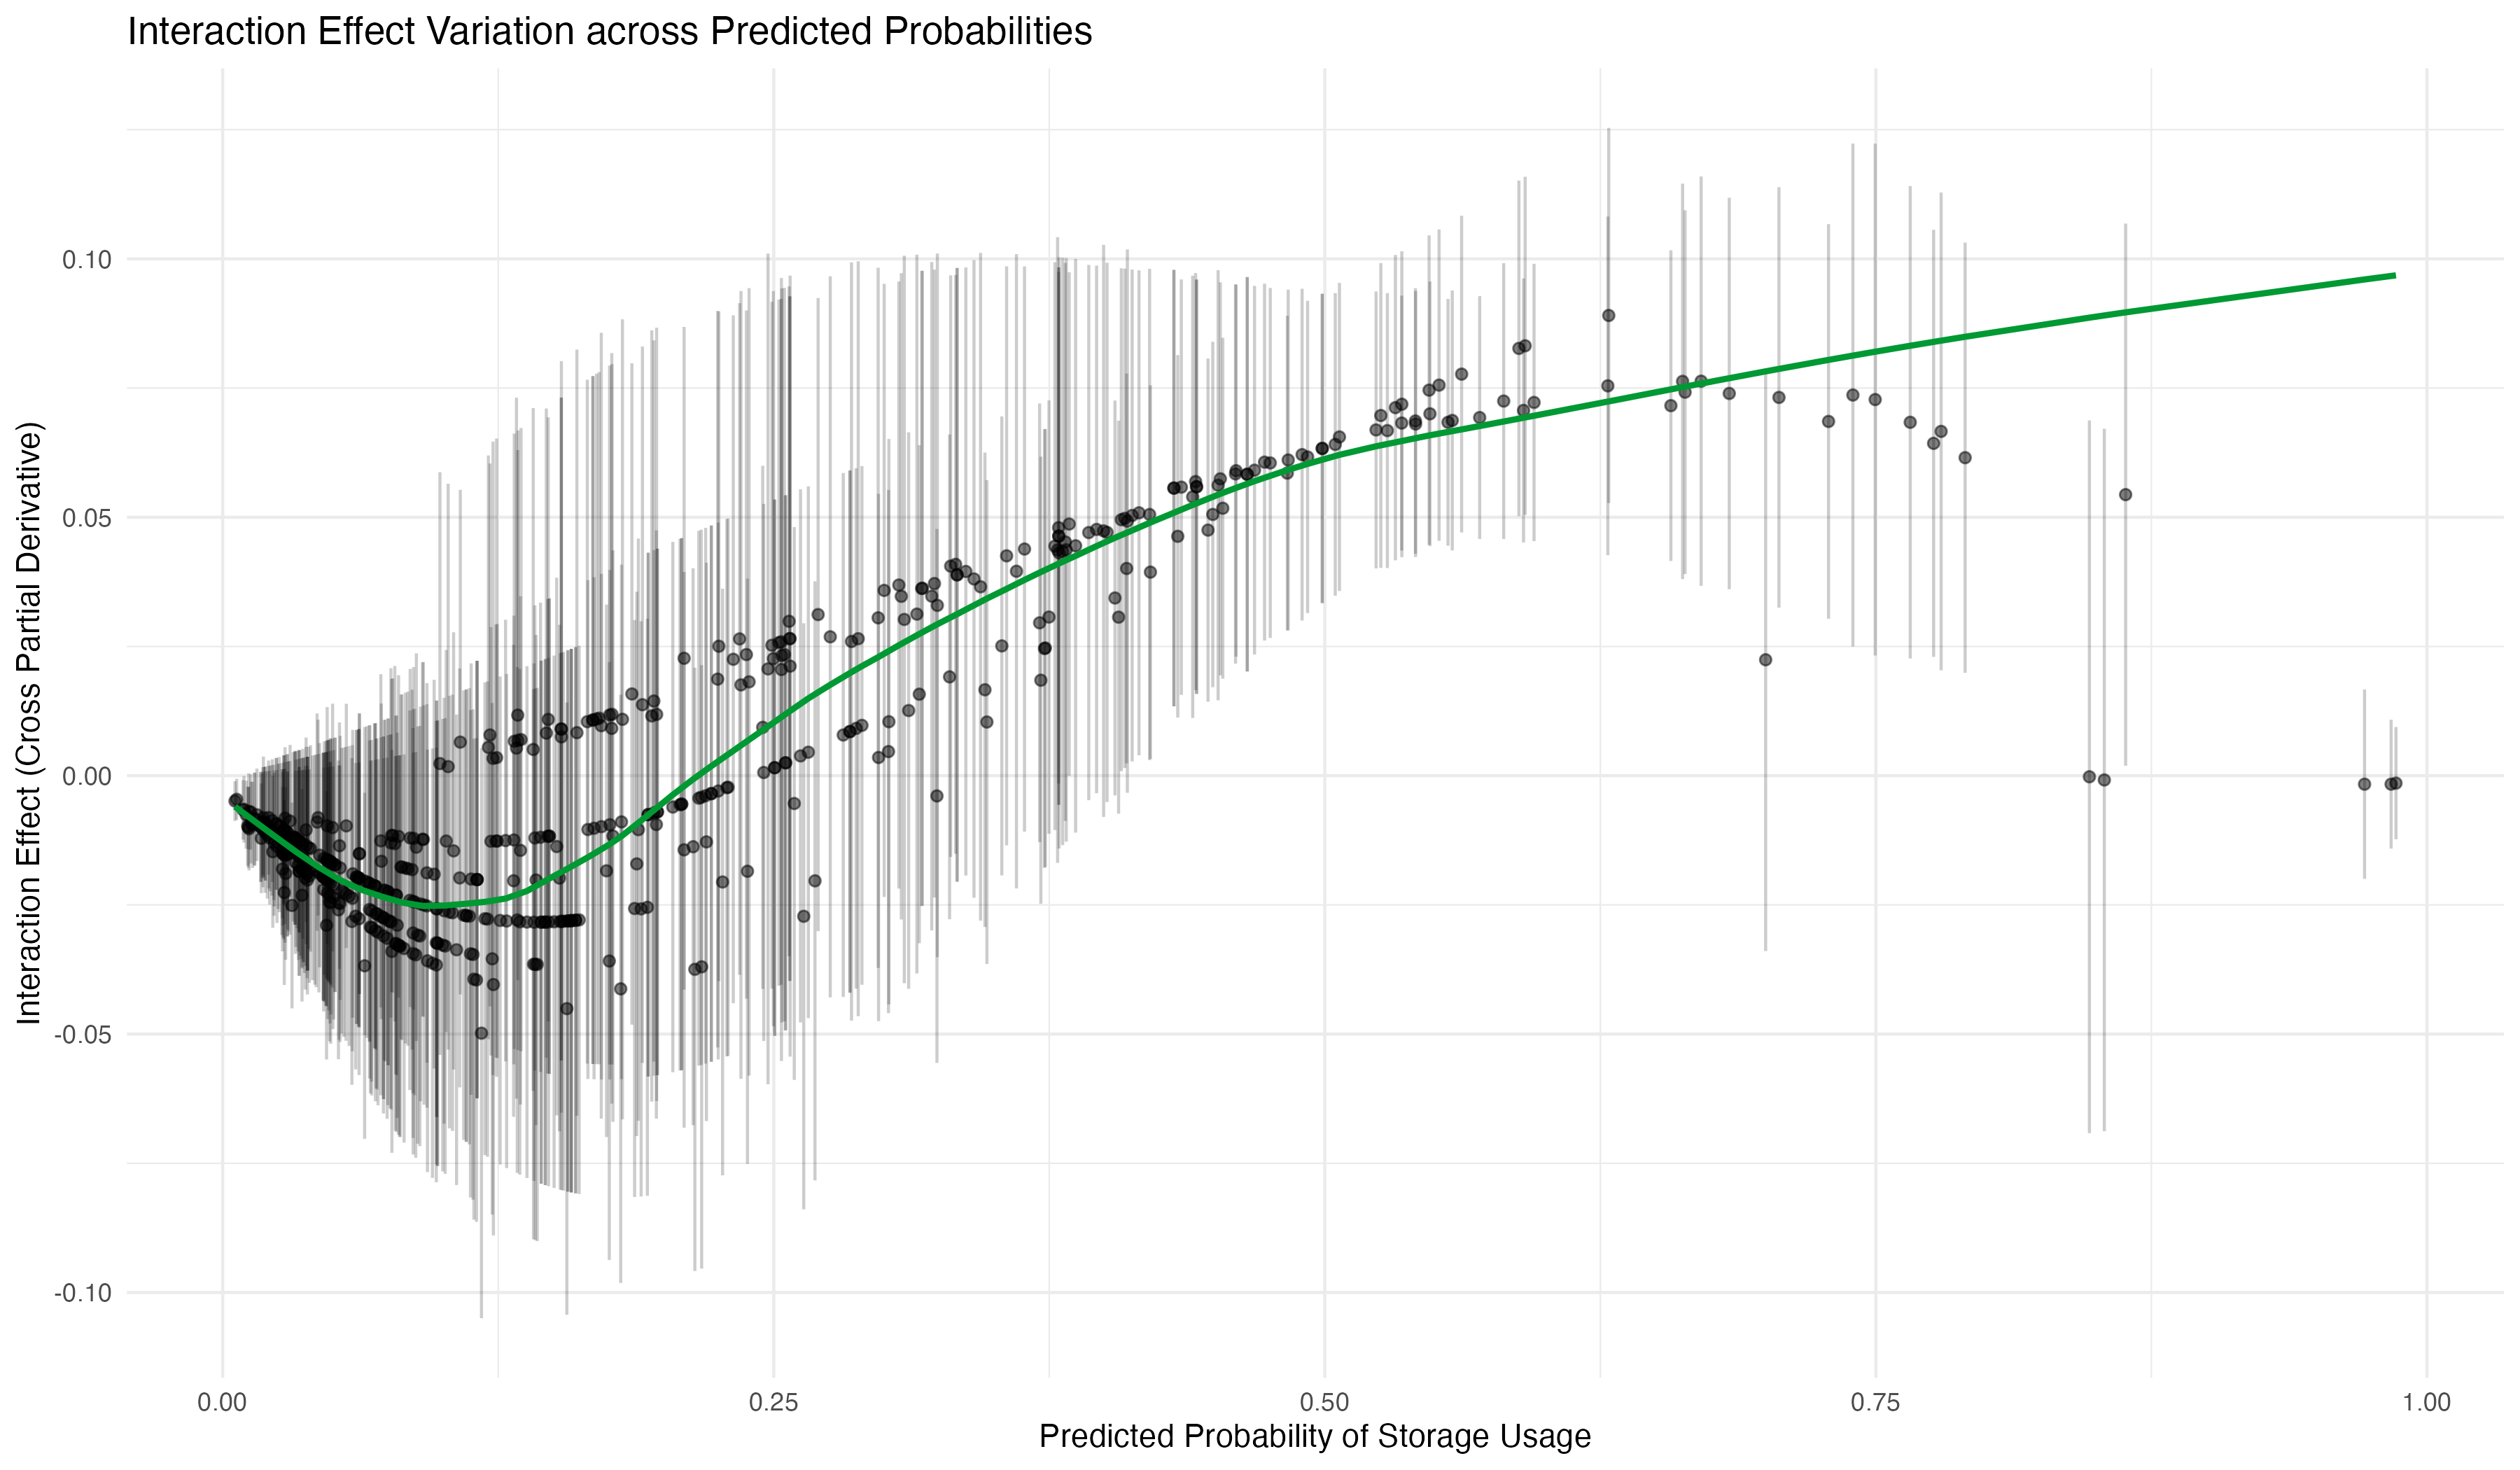
\includegraphics[width=1\textwidth]{figures/Interaction_Effect_across_Predicted Probabilities.png}
\caption{Interaction Effect Variation across Predicted Probability of Storage Usage}
\label{Figure: interaction effects}
\end{figure}

The results indicate that the relationship between the objective number of buyers and storage decisions is contingent on farmers' subjective beliefs about buyer competition. For farmers with low predicted probabilities of storage usage (generally below 0.15), the interaction effect tends to be negative, suggesting that the positive effect of additional buyers visiting at harvest diminishes when farmers perceive stronger buyer competition. Conversely, for farmers with higher predicted probabilities of storage usage, the interaction effect becomes positive, indicating that the combination of more buyers and stronger perceived competition reinforces storage decisions. This heterogeneity in the interaction effect underscores the complexity of farmers' decision-making processes regarding cold storage adoption, which are influenced by both market conditions and their perceptions thereof.

In addition, several demographic characteristics also influence storage decisions. Age negatively affects storage usage across all models, with coefficients ranging from -0.02 to -0.03. The effect is statistically significant, indicating that older individuals are less likely to engage in storage. Higher education levels positively influence storage decisions. The coefficients range from 0.31 to 0.38 and are statistically significant at the 5\% or 10\% level, suggesting that more educated individuals are more likely to use storage, potentially due to better access to information or greater financial literacy. Having a family member who ever served as a village leader significantly increases the likelihood of storage. The estimated coefficients range from 1.17 to 1.32 (p $<$ 0.01), indicating a strong positive effect. These people may be getting reduced storage costs for storage due to their family connections. This finding may reflect the role of social capital and influence in shaping economic behaviors.

Risk preferences also play a key role in storage decisions. The coefficient on CRRA-adjusted risk aversion is consistently negative and highly significant across all models, ranging from -0.96 to -1.15. This result suggests that more risk-averse individuals are significantly less likely to store, which aligns with economic theory predicting that risk-averse agents prefer immediate sales over storage due to uncertainty in future prices.

These findings highlight the central role of farmers' subjective beliefs about buyers' competition in influencing storage decisions. The minimal impact of the actual number of buyers at harvest suggests that farmers respond more strongly to their perceptions of market conditions than to objective reality. Additionally, risk preferences, education, and social capital play significant roles in shaping storage behavior.



\subsubsection{Expected Buyer Movement and Storage Decisions}

\noindent This section analyzes the impact of farmers' expectations regarding buyer availability and competitiveness in three months on their storage decisions. The key independent variables capture whether farmers anticipate more buyers, fewer buyers, or no change in buyer numbers post-harvest. The logistic regression model, incorporating town-level fixed effects, is specified as follows:

\begin{equation}
    \text{logit} \left( P(S_i = 1) \right) = \alpha_0 + \alpha_1 E^m_i + \alpha_2 E^f_i + \alpha_3 X_i + \gamma_t + \varepsilon_i,
\end{equation}

where $E^m_i$ denotes the expectation of more buyers, $E^f_i$ represents the expectation of fewer buyers, and $X_i$ includes demographic controls. Town-level fixed effects are denoted by $\gamma_t$, and $\varepsilon_i$ is the error term.


% Table created by stargazer v.5.2.3 by Marek Hlavac, Social Policy Institute. E-mail: marek.hlavac at gmail.com
% Date and time: Tue, Feb 25, 2025 - 23:06:15
\begin{table}[!htbp] \centering 
  \caption{} 
  \label{tab: binary storage ~ farmer's expectation on movement} 
\begin{tabular}{@{\extracolsep{5pt}}lcc} 
\\[-1.8ex]\hline 
\hline \\[-1.8ex] 
 & \multicolumn{2}{c}{\textit{Dependent variable:}} \\ 
\cline{2-3} 
\\[-1.8ex] & \multicolumn{2}{c}{Storage Usage (Binary)} \\ 
\\[-1.8ex] & (1) & (2)\\ 
\hline \\[-1.8ex] 
 Fewer Buyers & 0.43 & 0.37 \\ 
  & (0.32) & (0.34) \\ 
  & & \\ 
 More Buyers & 2.71$^{***}$ & 2.78$^{***}$ \\ 
  & (0.38) & (0.39) \\ 
  & & \\ 
 Age & $-$0.04$^{*}$ & $-$0.03$^{*}$ \\ 
  & (0.01) & (0.01) \\ 
  & & \\ 
 Education & 0.26 & 0.18 \\ 
  & (0.19) & (0.20) \\ 
  & & \\ 
 Family Leader & 1.10$^{**}$ & 1.04$^{**}$ \\ 
  & (0.36) & (0.39) \\ 
  & & \\ 
 CRRA Adjusted & $-$1.14$^{***}$ & $-$1.00$^{**}$ \\ 
  & (0.33) & (0.34) \\ 
  & & \\ 
 Num Buyers &  & 0.45$^{***}$ \\ 
  &  & (0.11) \\ 
  & & \\ 
 Subjective Belief &  & $-$1.70$^{***}$ \\ 
  &  & (0.32) \\ 
  & & \\ 
 Constant & 0.95 & 4.51$^{***}$ \\ 
  & (0.94) & (1.21) \\ 
  & & \\ 
\hline \\[-1.8ex] 
Town Fixed Effects & Yes & Yes \\ 
Observations & 549 & 549 \\ 
Log Likelihood & $-$189.39 & $-$173.22 \\ 
Akaike Inf. Crit. & 406.79 & 378.44 \\ 
\hline 
\hline \\[-1.8ex] 
\textit{Note:}  & \multicolumn{2}{r}{$^{*}$p$<$0.05; $^{**}$p$<$0.01; $^{***}$p$<$0.001} \\ 
\end{tabular} 
\end{table} 


The results in Table \ref{tab: binary storage ~ farmer's expectation on movement} indicate that farmers who anticipate an increase in the number of buyers within three months are significantly more likely to store their harvest. This is evident from the strong and statistically significant coefficients on $E^m_i$ (2.71 in Model 1 and 2.78 in Model 2), highlighting a robust positive effect. This suggests that expectations of heightened buyers' competitiveness at a later stage motivate farmers to delay sales, anticipating that intensified competition among buyers will lead to higher farm-gate prices. Such behavior is consistent with intertemporal optimization, where farmers strategically hold onto their produce to maximize returns when they expect stronger buyer competition in the near future.  

Conversely, expectations of fewer buyers ($E^f_i$) yield positive but statistically insignificant coefficients. A priori, one might expect that pessimistic market expectations would discourage storage, as farmers anticipating reduced buyer competition may prefer immediate sales to avoid potential price declines. However, the lack of statistical significance suggests that these expectations do not systematically influence storage decisions. Several factors could explain this result. As illustrated in the first chapter and the previous section, the existence of buyer collusion could attenuate the importance of the number of buyers as a measure of competition. For instance, farmers may not perceive a decline in buyer numbers as an unambiguous signal of lower prices, particularly if they believe that remaining buyers will still offer competitive prices. Additionally, liquidity constraints, risk aversion, and implicit storage costs could weaken the direct relationship between pessimistic expectations and storage behavior.  

These findings reveal an asymmetry in how farmers respond to expected changes in buyers' competitiveness. While the anticipation of more intense buyer competition strongly incentivizes storage, expectations of reduced competition do not significantly deter it. This suggests that farmers are more sensitive to potential price gains from increased buyer competition than to potential risks associated with fewer buyers, emphasizing the role of perceived future market opportunities in shaping storage decisions.


Table \ref{tab:predicted_probs} further presents the predicted probabilities of storage usage based on farmers’ expectations regarding buyer numbers in three months. Farmers who expect no change in buyer numbers exhibit a predicted probability of 0.201, while those anticipating fewer buyers have a slightly higher probability of 0.249. Notably, farmers expecting more buyers have a predicted probability of 0.562, indicating a strong inclination toward storage when they anticipate heightened buyer competition. This substantial difference suggests that expectations of intensified competition at harvest play a crucial role in storage decisions. Figure \ref{Figure: Difference-from-Baseline Plot} visualizes these differences, illustrating that the increase in predicted probability for those expecting more buyers is both economically meaningful and statistically significant.


% latex table generated in R 4.4.2 by xtable 1.8-4 package
% Tue Mar  4 20:06:09 2025
\begin{table}[htbp]
\centering
\begin{tabular}{lrrrr}
  \hline
expect\_3\_months & avg\_prob & se & CI\_lower & CI\_upper \\ 
  \hline
no\_change & 0.211 & 0.032 & 0.148 & 0.273 \\ 
  fewer\_buyers & 0.259 & 0.042 & 0.178 & 0.341 \\ 
  more\_buyers & 0.572 & 0.064 & 0.446 & 0.698 \\ 
   \hline
\end{tabular}
\caption{Predicted Probabilities of Storage by Expected Buyers} 
\label{tab:predicted_probs}
\end{table}



\begin{figure}[htbp]
    \centering
    \begin{subfigure}{\textwidth}
        \centering
        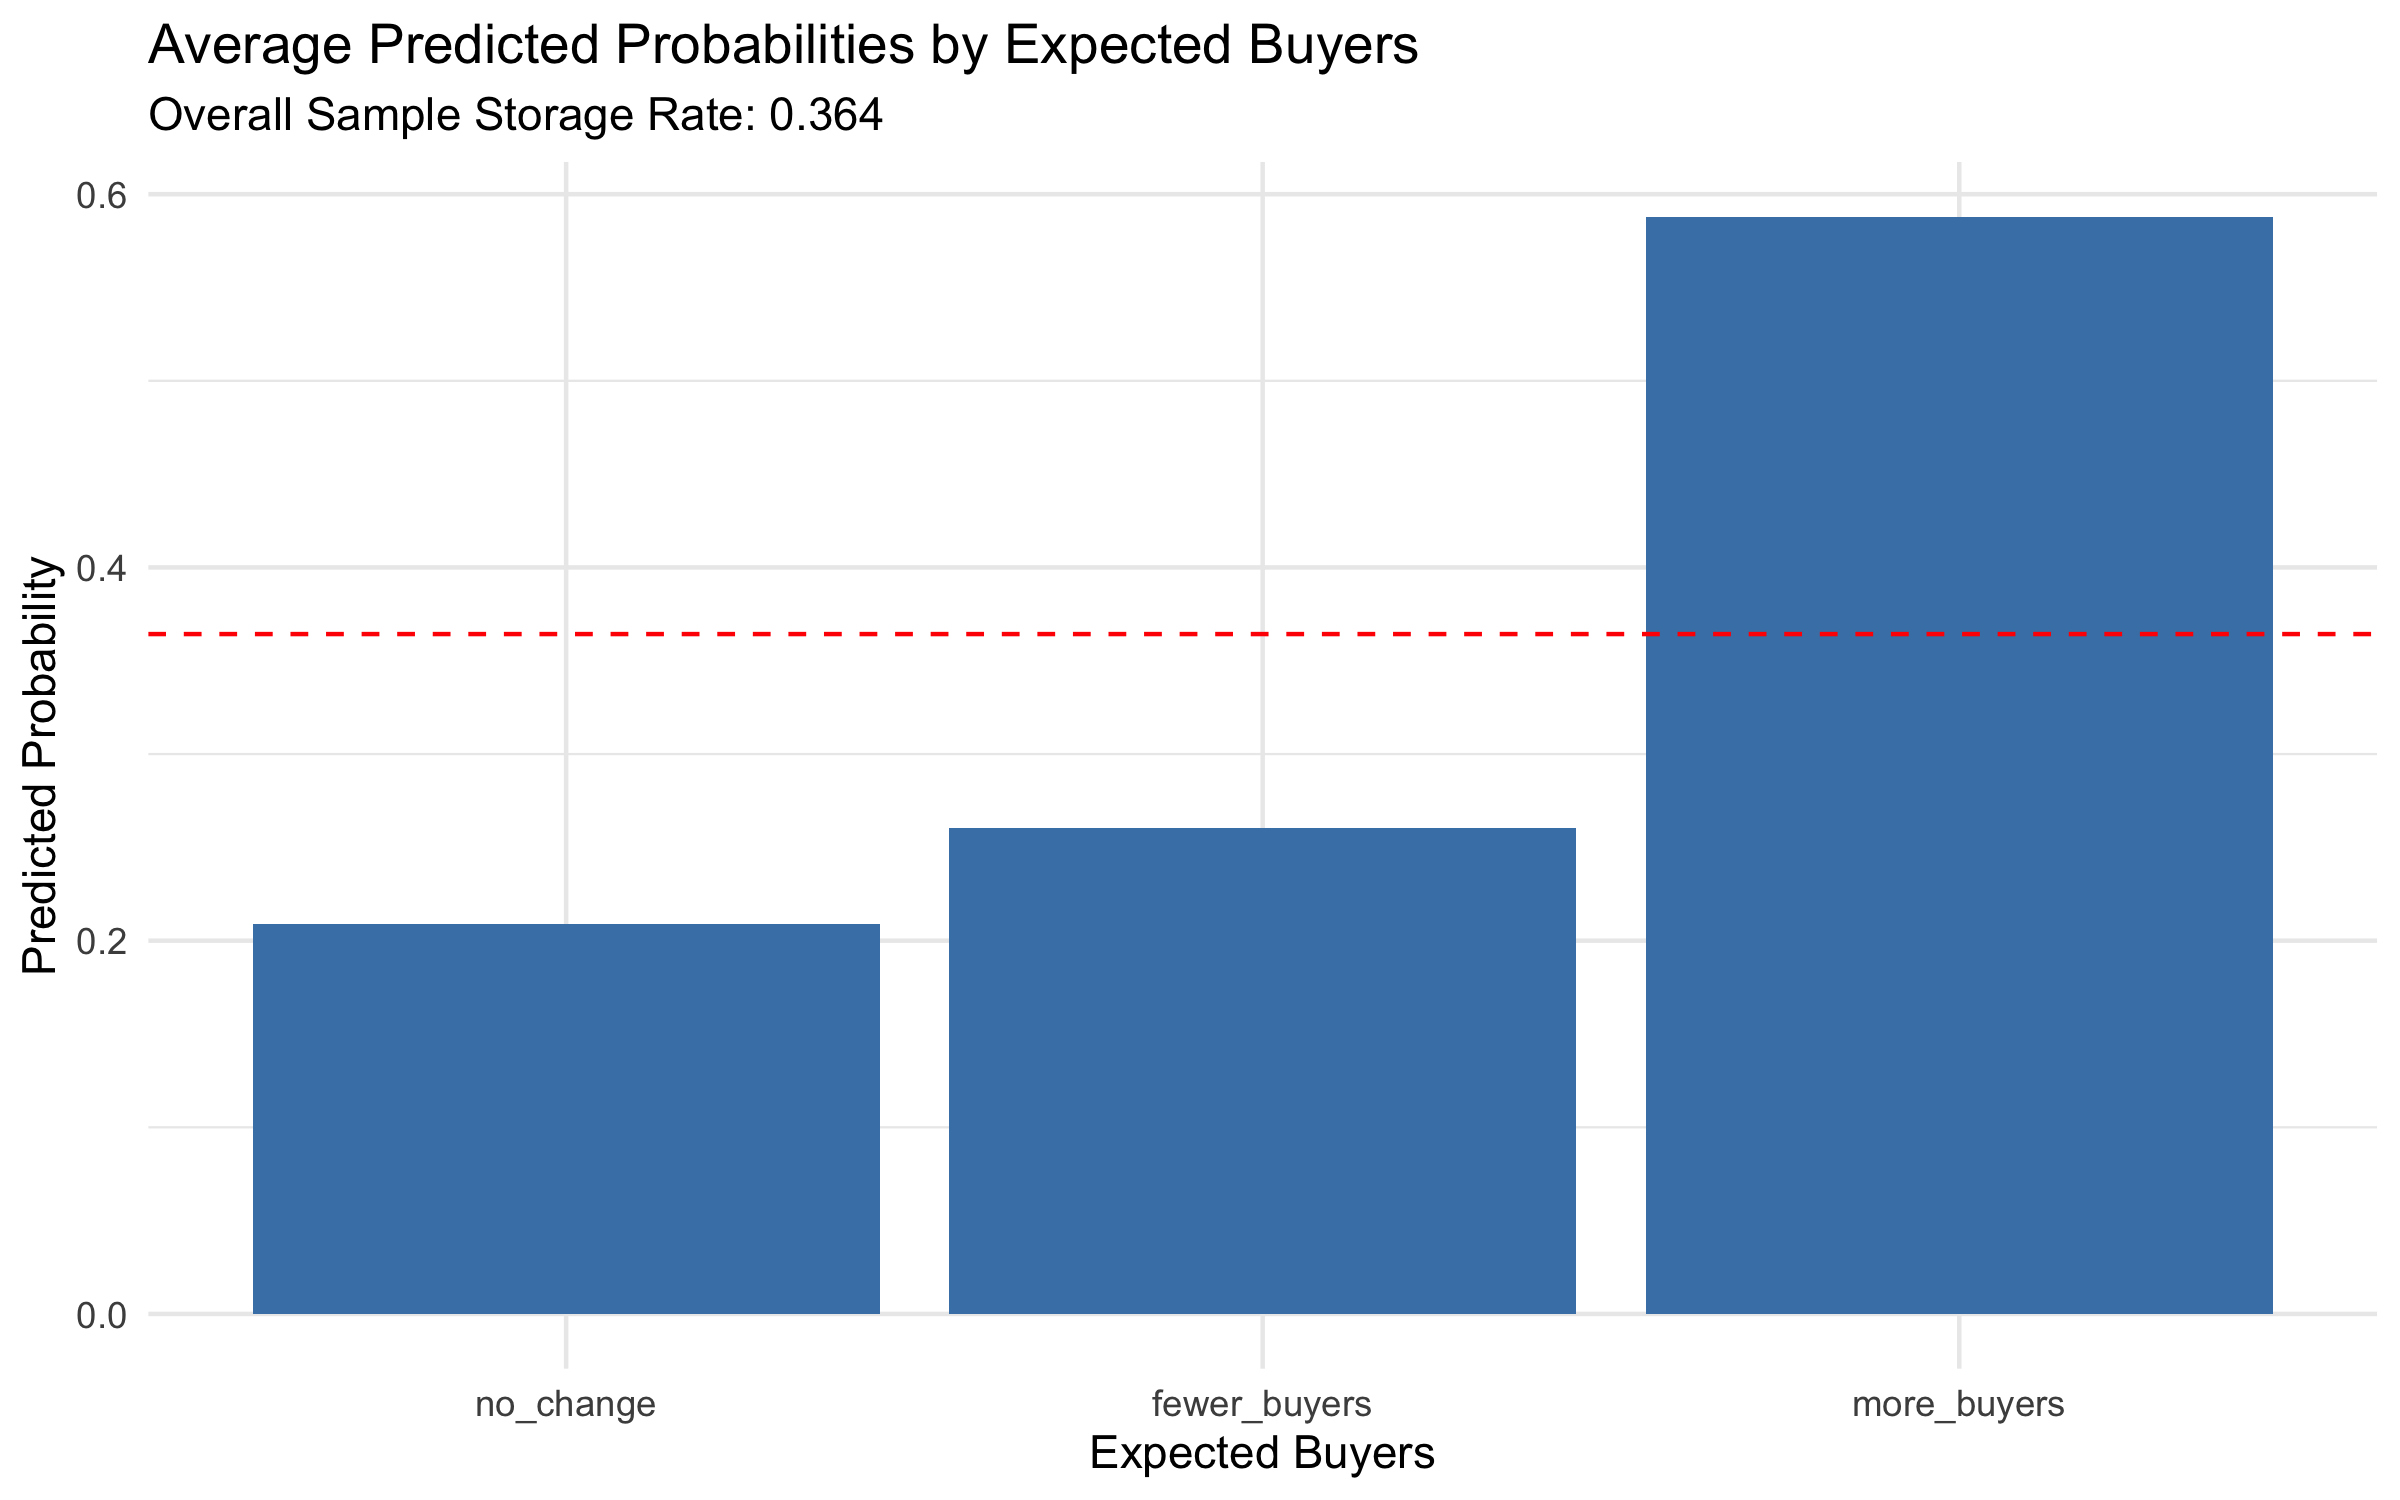
\includegraphics[height=0.28\textheight]{figures/overall_predicted_probs.png}
        \caption{}
    \end{subfigure}\\[2mm]
    
    \begin{subfigure}{\textwidth}
        \centering
        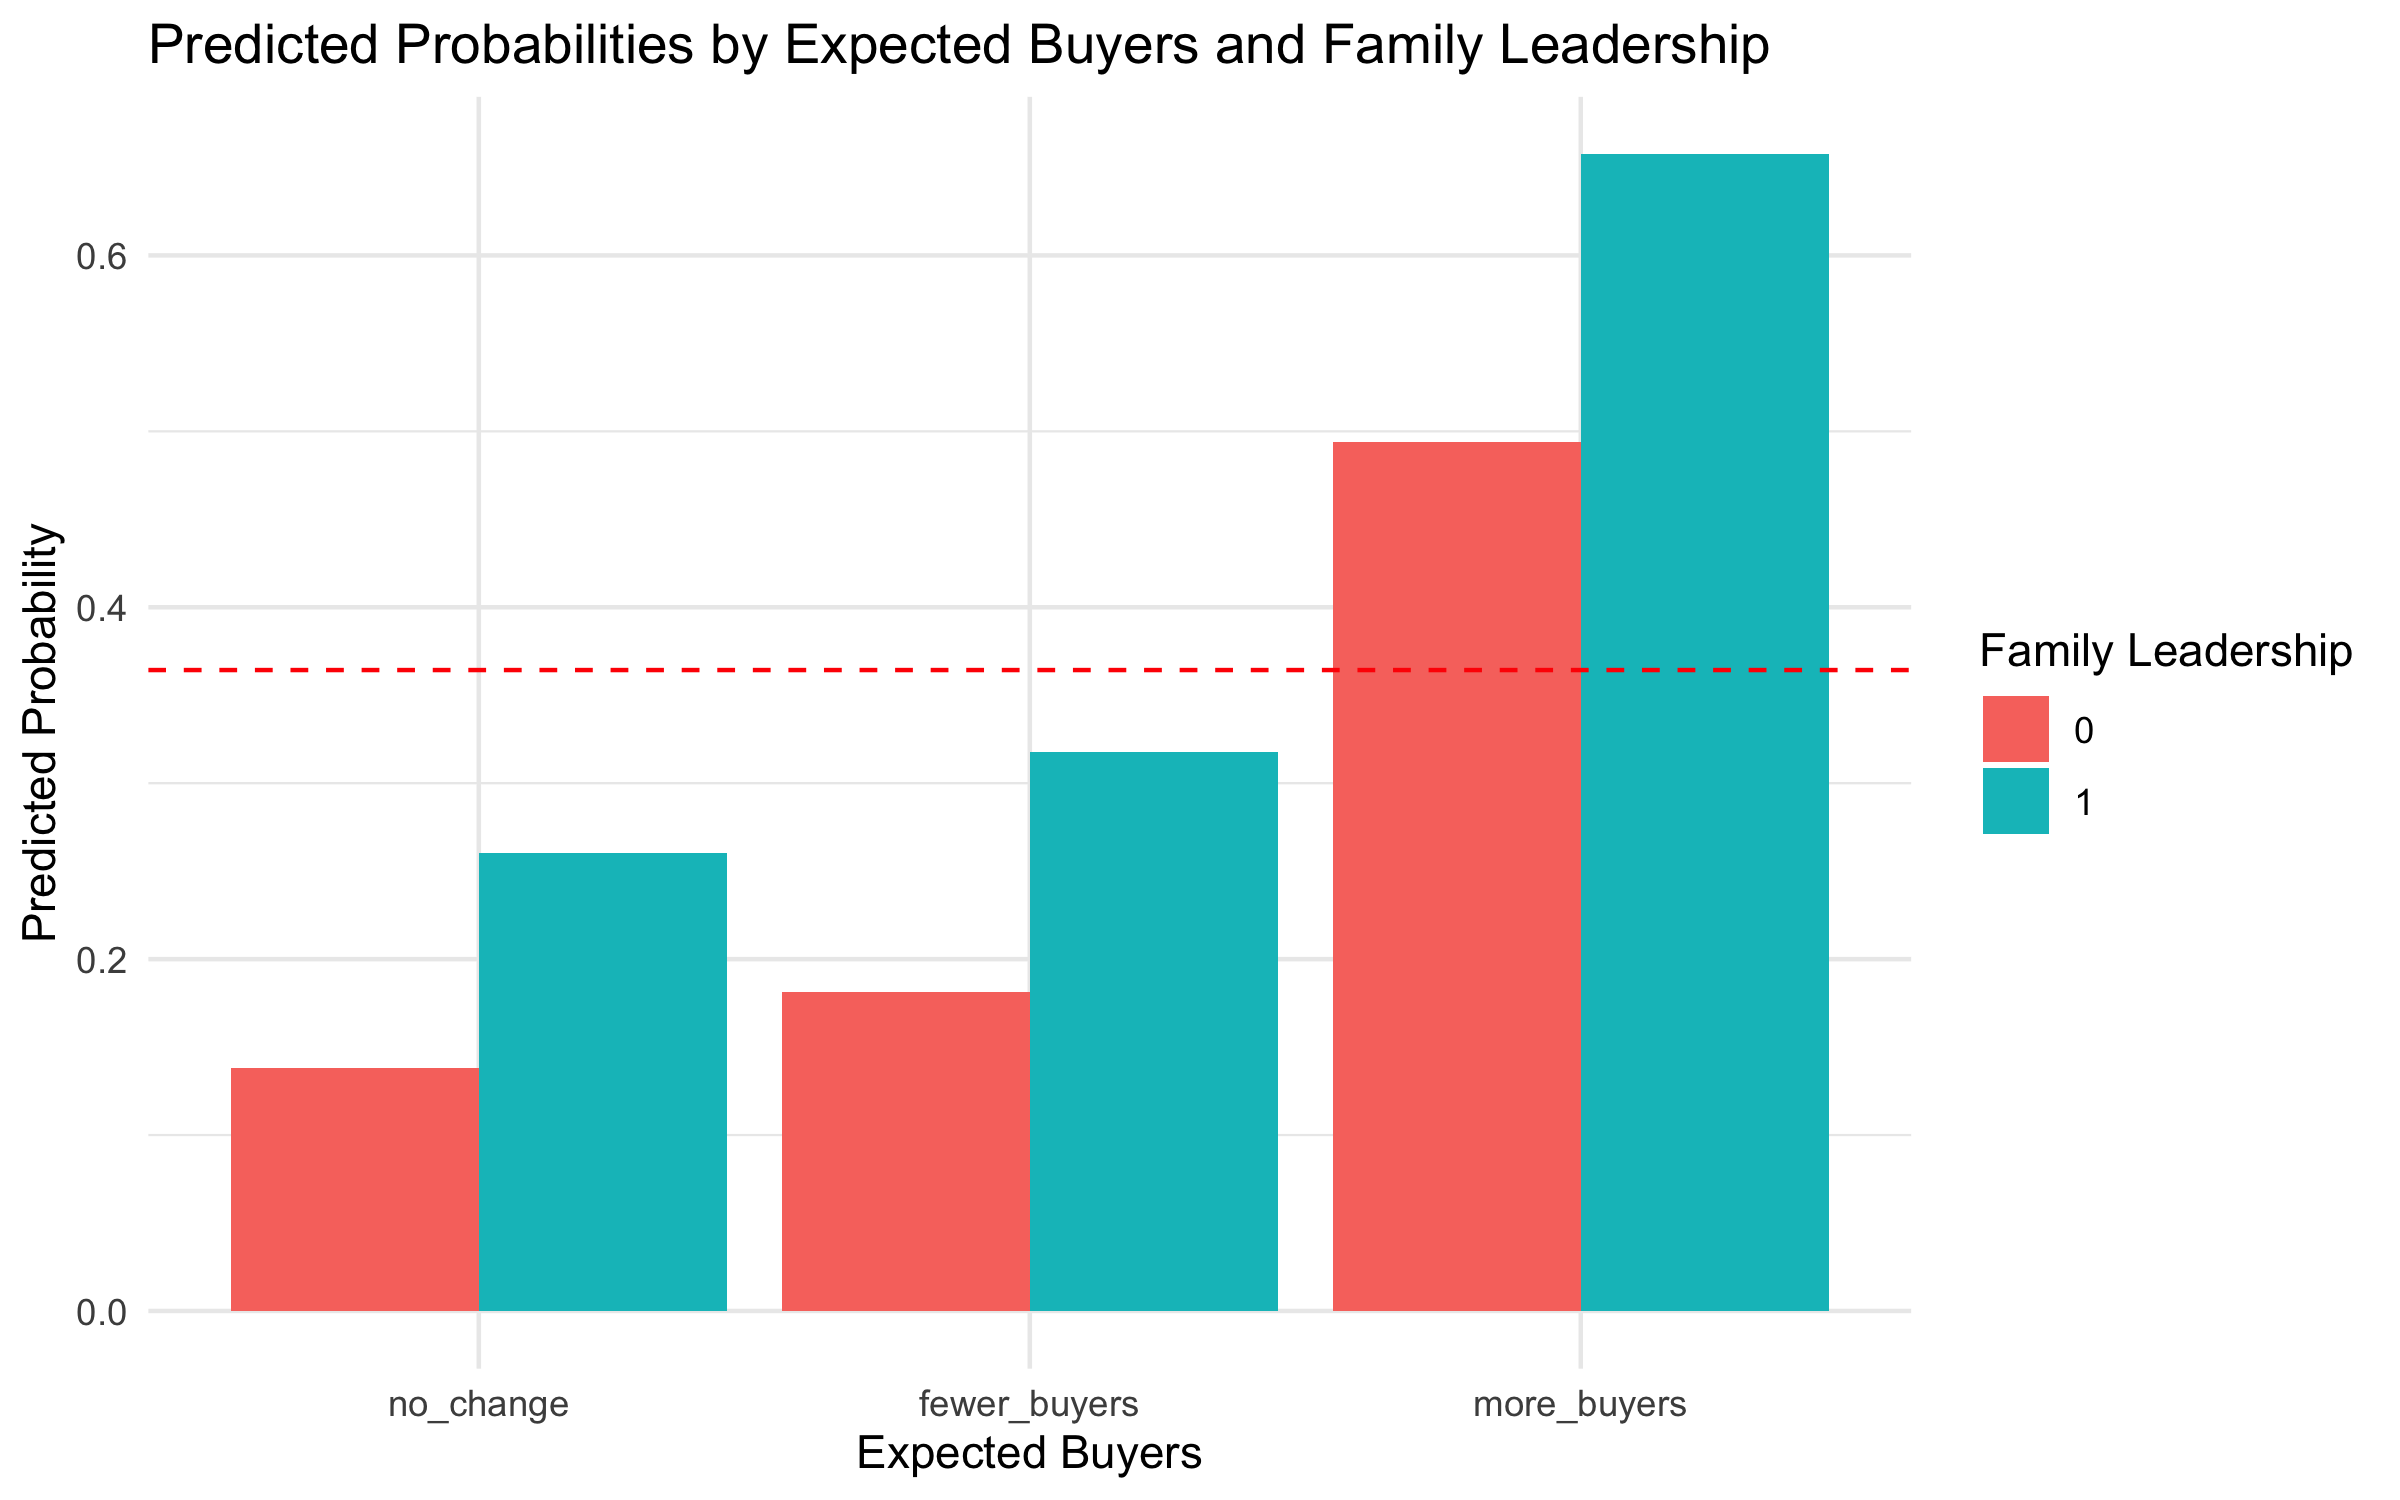
\includegraphics[height=0.28\textheight]{figures/predicted_probs_by_family.png}
        \caption{}
    \end{subfigure}\\[2mm]

    \begin{subfigure}{\textwidth}
        \centering
        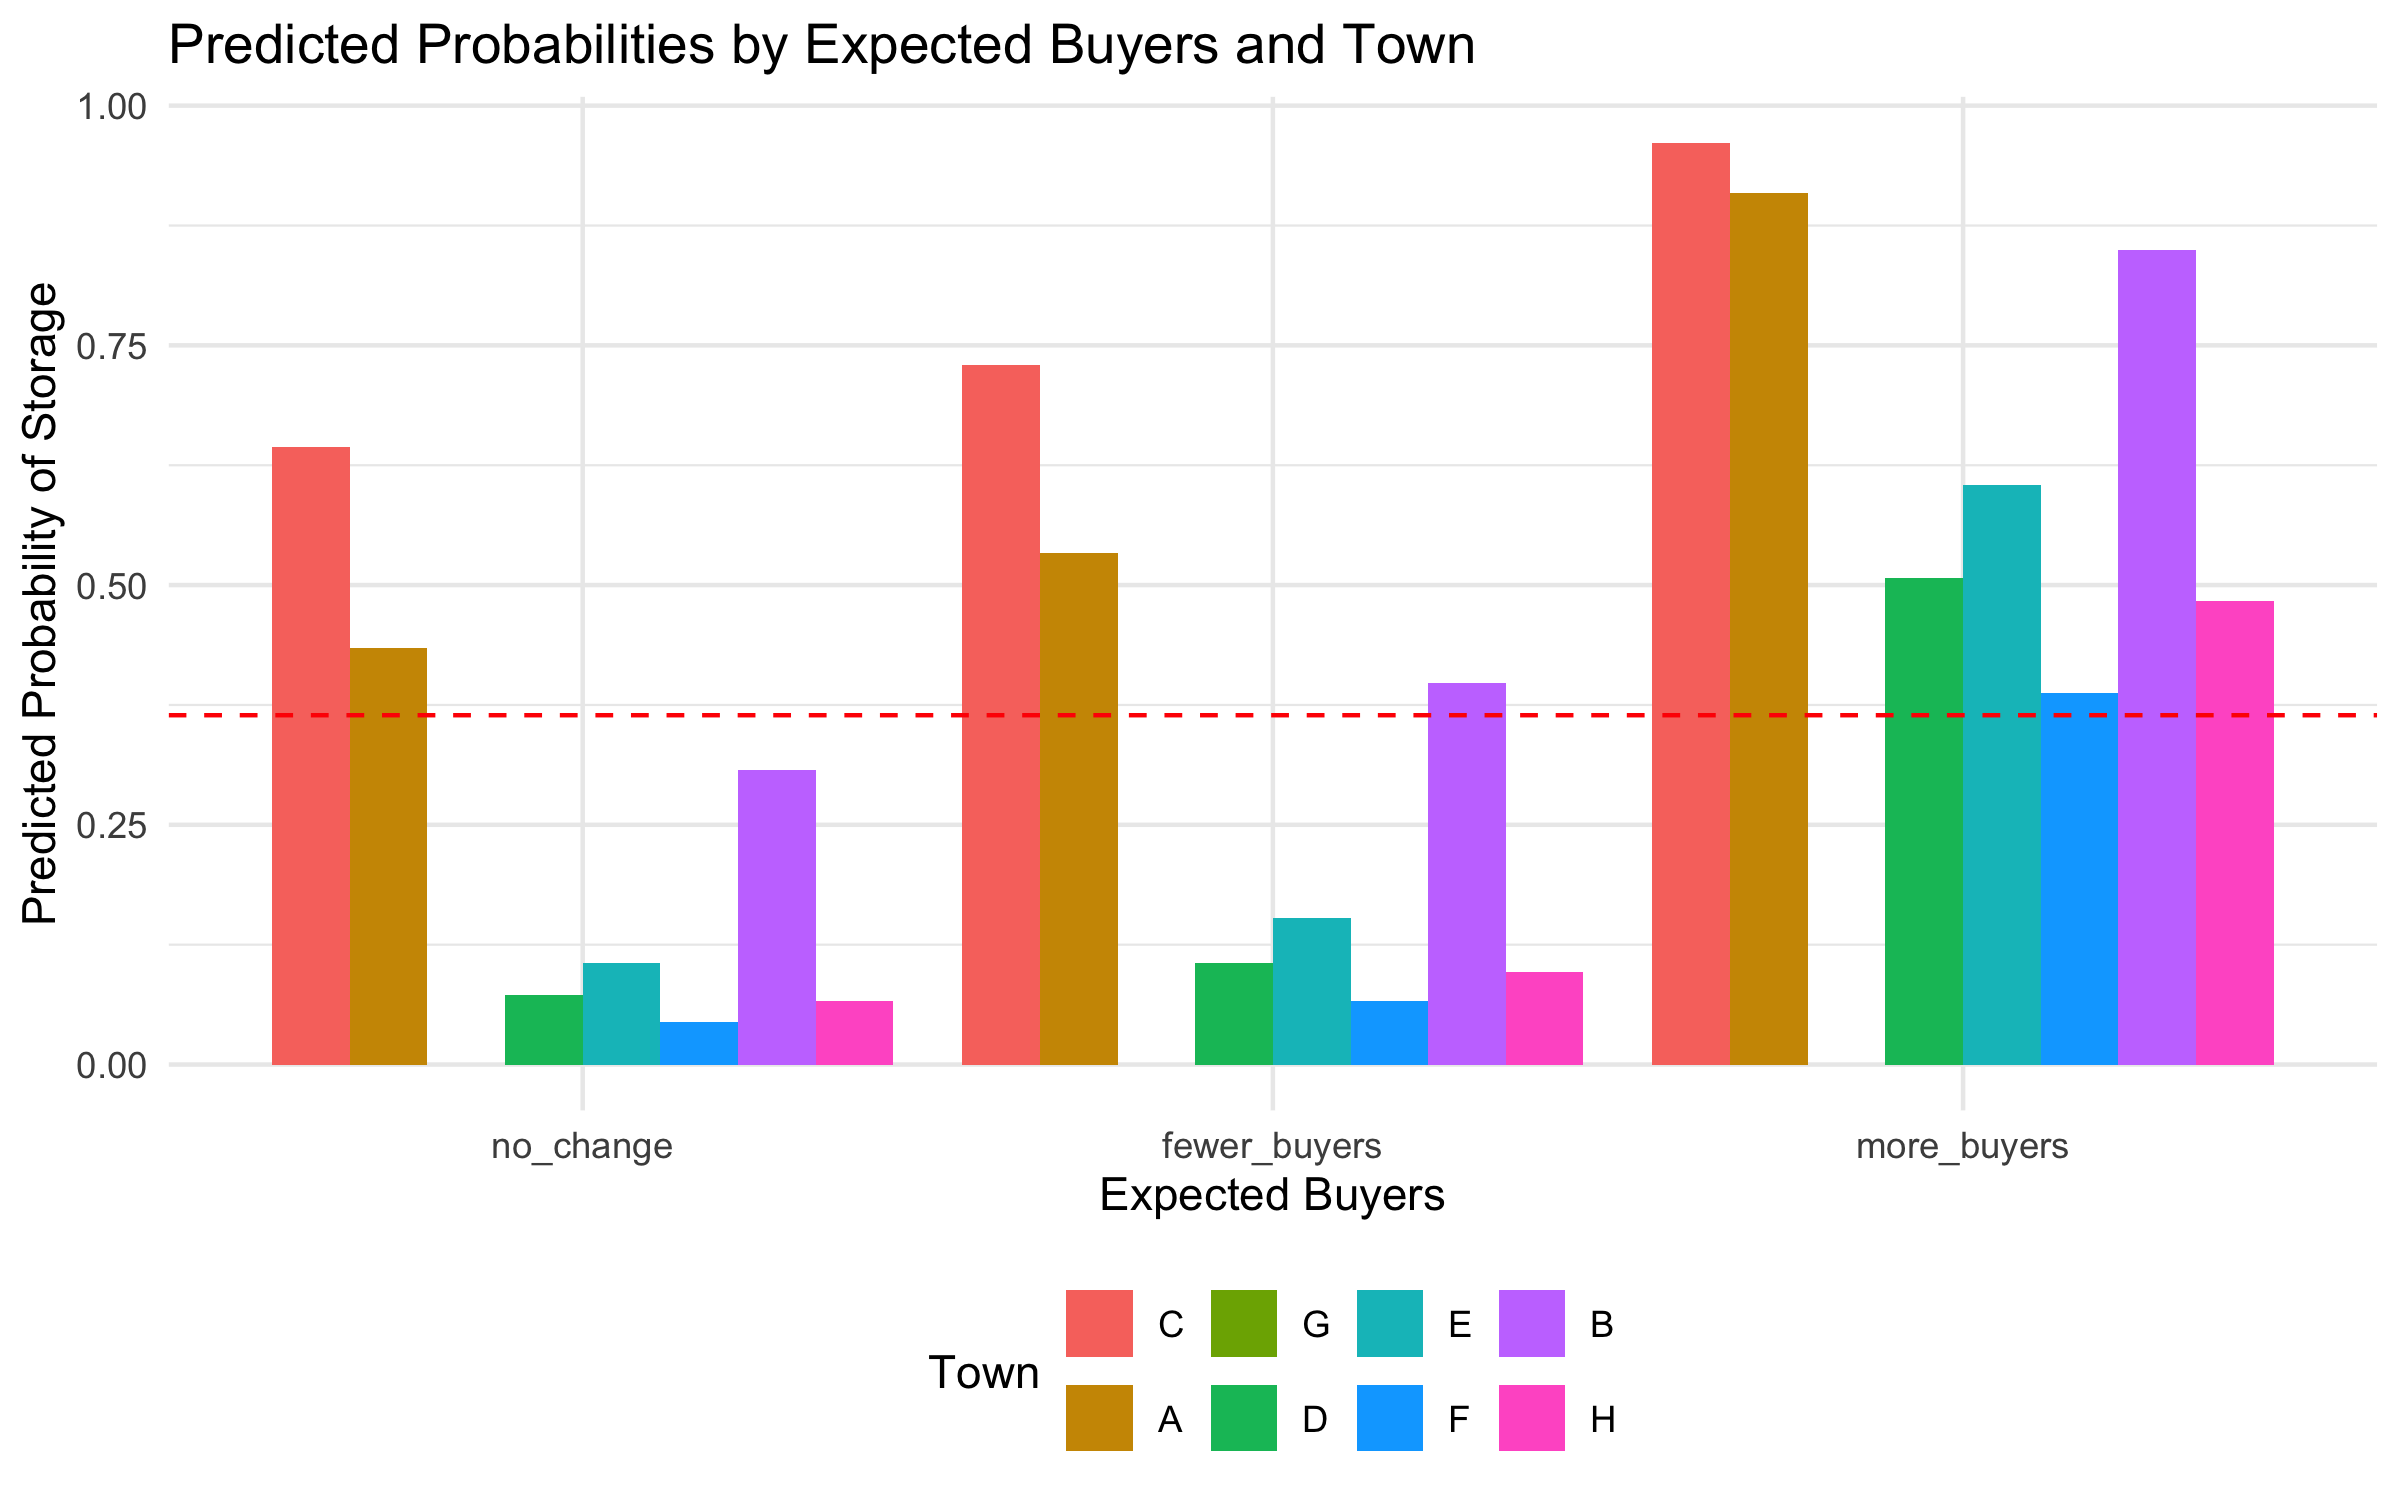
\includegraphics[height=0.28\textheight]{figures/predicted_probs_by_town.png}
        \caption{}
    \end{subfigure}


    \caption{Predicted Probabilities of Storage Usage by Expected Buyer Movement}
    \label{fig:three-images}
\end{figure}





\begin{figure}[ht]
    \centering
    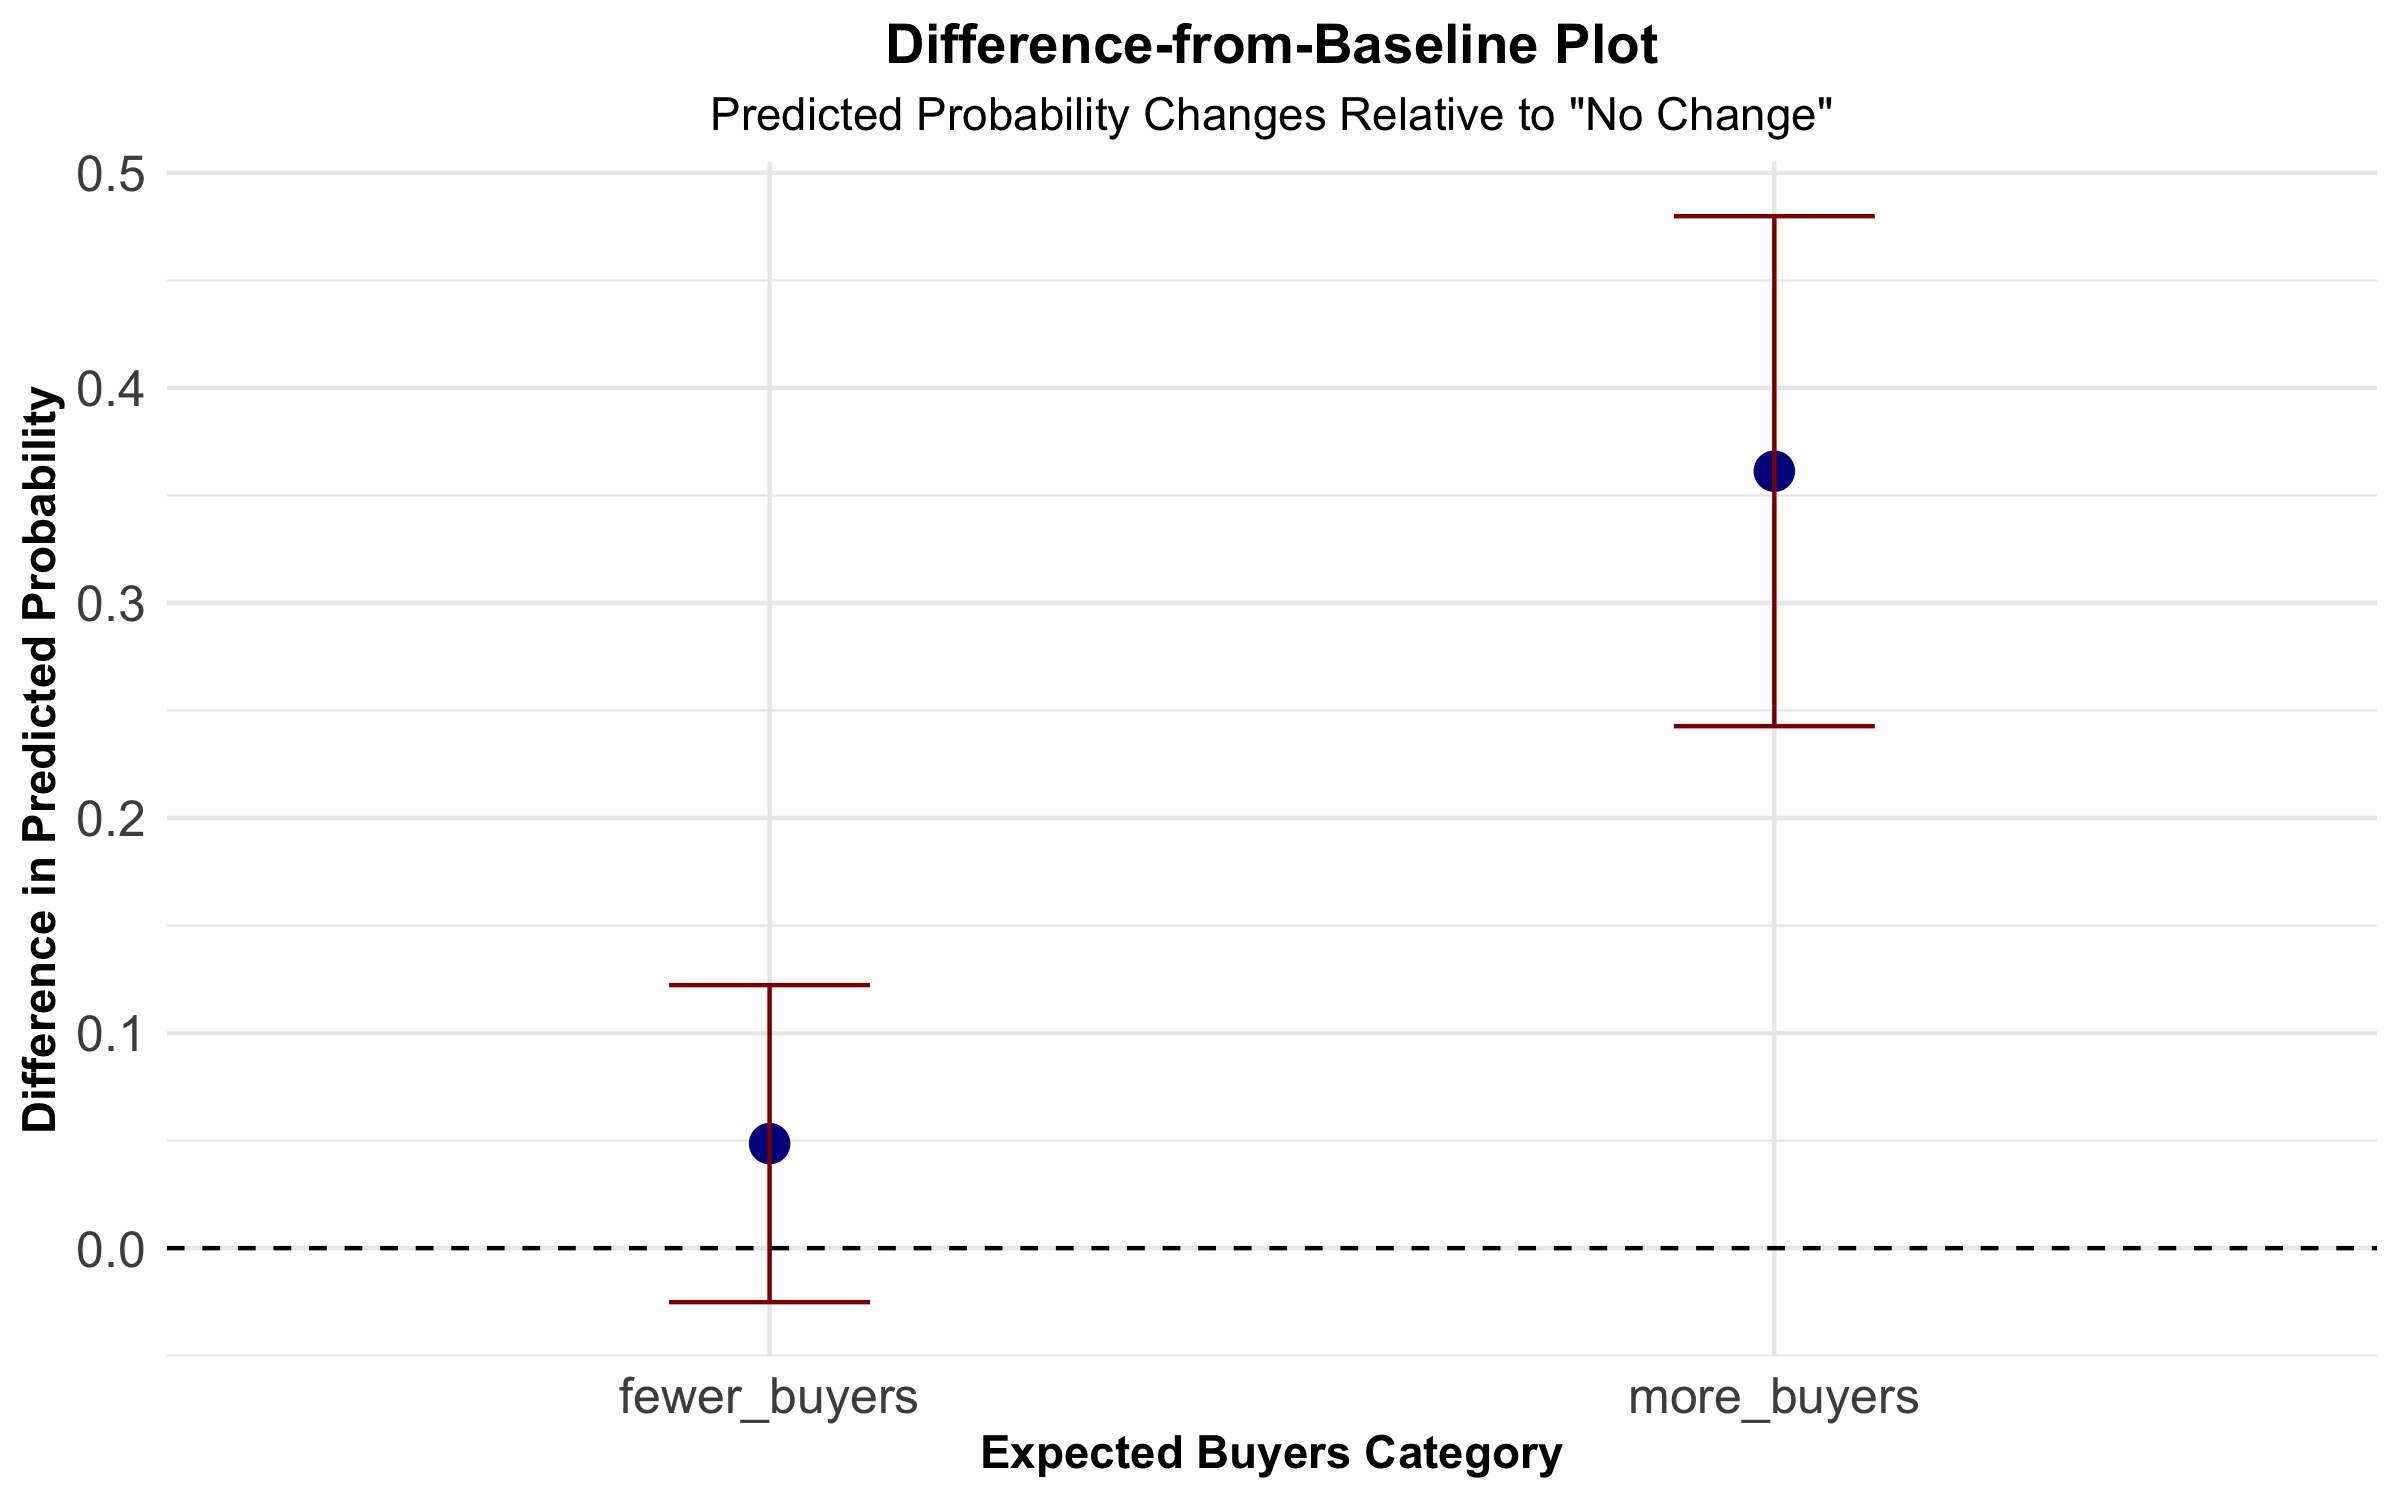
\includegraphics[width=1\textwidth]{figures/filtered_difference_from_baseline_plot.png}
    \caption{Difference-from-Baseline Plot}
    \label{Figure: Difference-from-Baseline Plot}
\end{figure}

\newpage
\begin{figure}[ht]
\centering
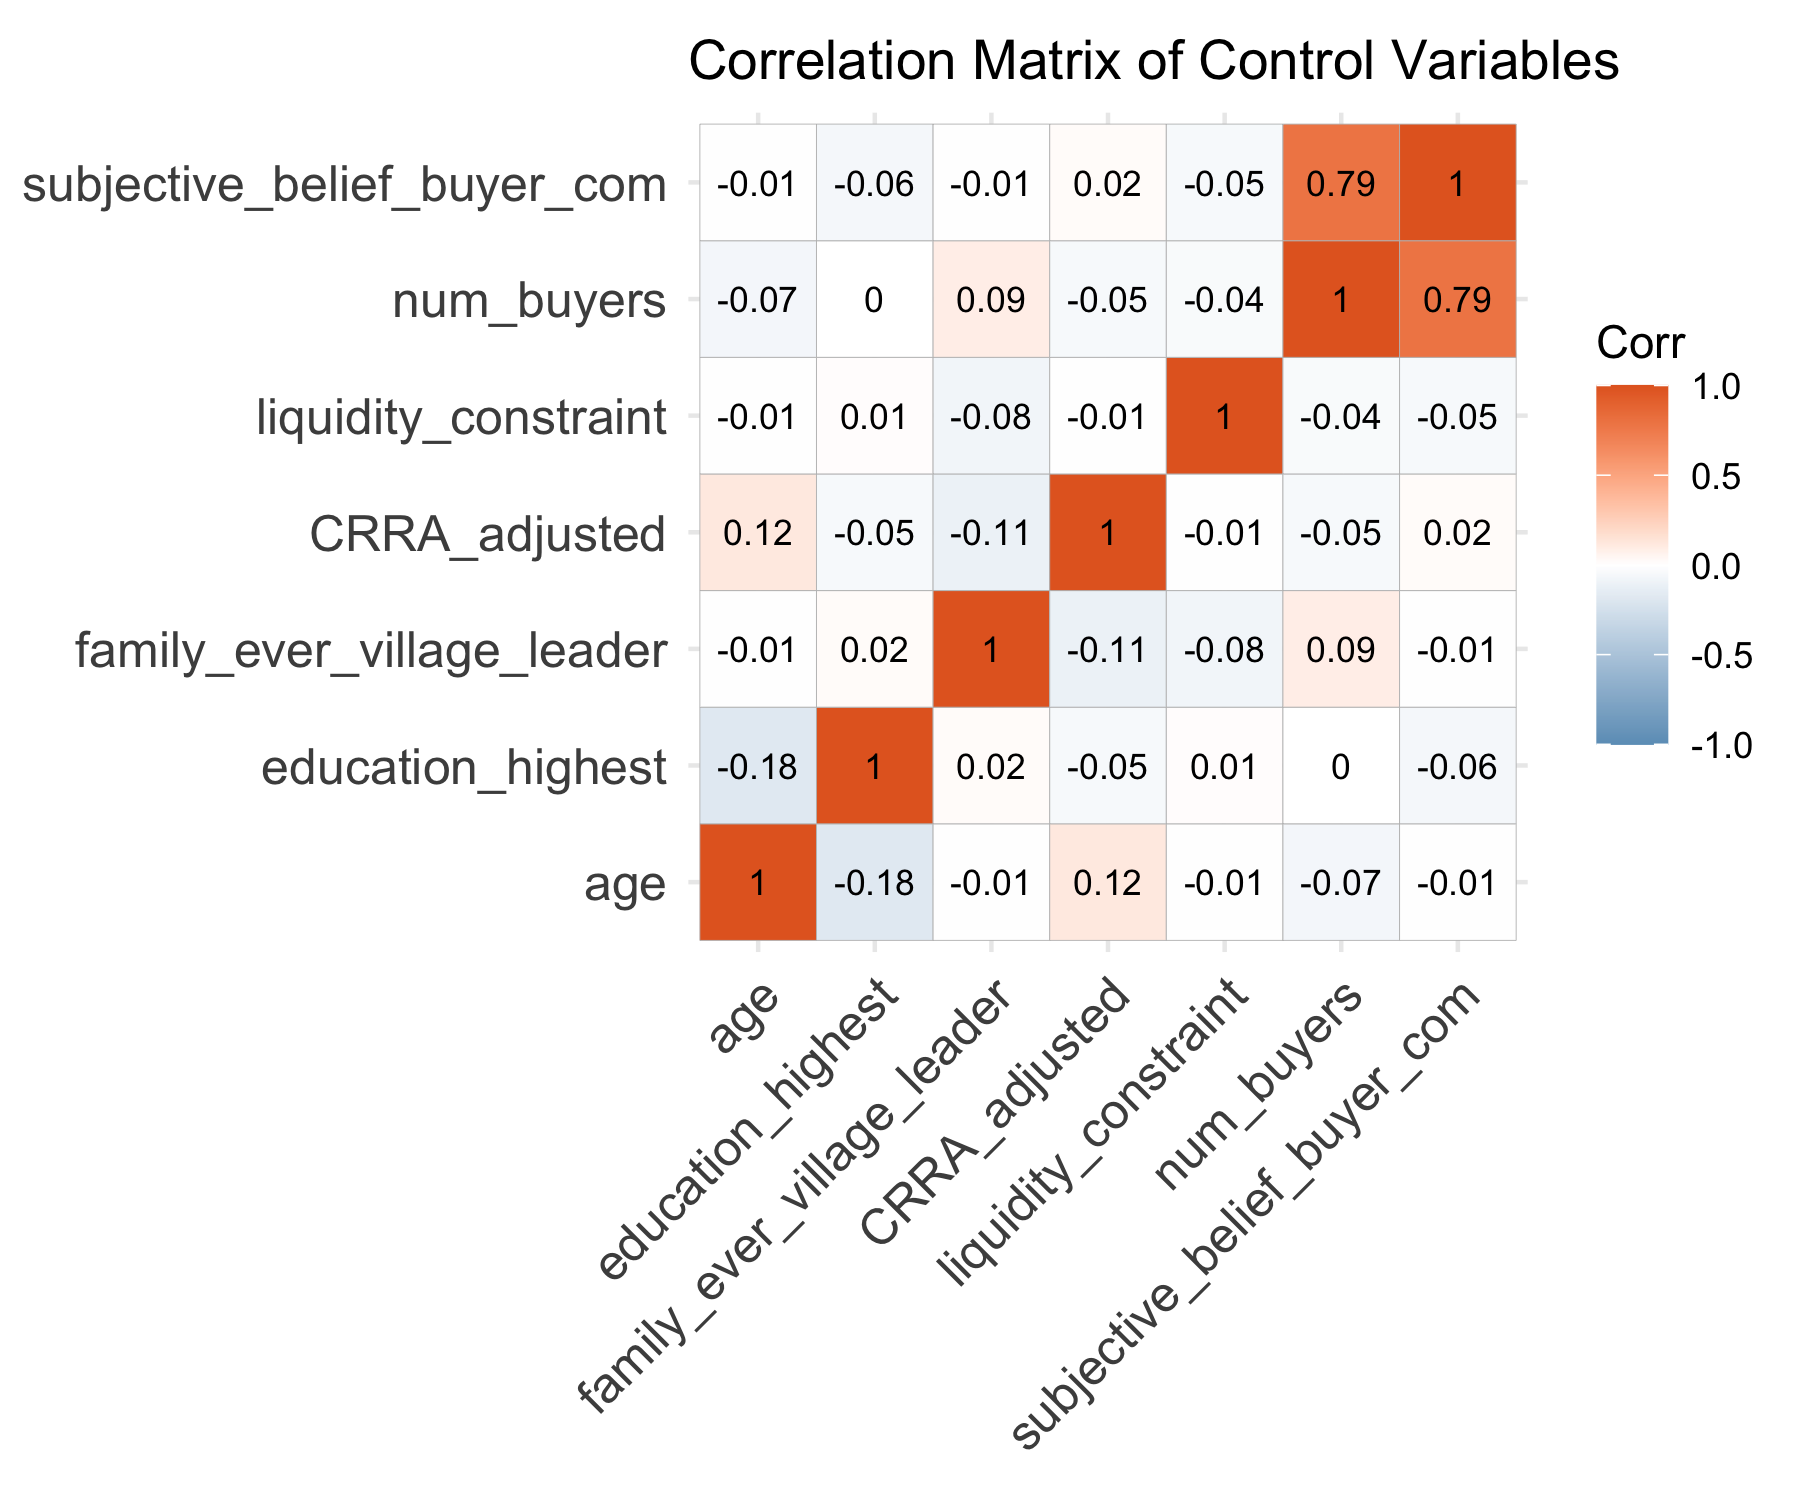
\includegraphics[width=1\textwidth]{figures/correlation_matrix_controls.png}
\caption{Correlation Matrix of Controls}
\label{Figure: Correlation Matrix of Controls}
\end{figure}

Demographic and risk-related factors continue to influence storage decisions in expected directions. Age negatively affects storage usage, with coefficients of -0.04 and -0.03, indicating that older individuals are less likely to store. Family leadership status remains a strong positive predictor, with coefficients of 1.10 and 1.04. Risk aversion exerts a significant negative effect, with coefficients of -1.14 and -1.00, reinforcing the tendency of risk-averse individuals to favor immediate sales over storage.  

The correlation matrix of control variables, presented in Figure \ref{Figure: Correlation Matrix of Controls}, further contextualizes these findings by illustrating the relationships among key covariates. The negative correlation between age and education level ($\rho = -0.18$) aligns with the observed effect of age on storage behavior, as younger farmers—who tend to have higher education—may be more receptive to market-based strategies such as storage. Similarly, the relatively low correlation between risk aversion (CRRA adjusted) and other covariates suggests that its influence on storage decisions operates independently of other demographic characteristics. Additionally, farmers’ subjective beliefs about buyer competition at harvest exhibit a strong positive correlation with the objective number of buyers ($\rho = 0.79$), reinforcing the idea that perceptions align with reality to a significant extent but remain distinct factors. The overall low to moderate correlations among control variables alleviate concerns about multicollinearity, supporting the reliability of the logistic regression estimates above. 


\newpage
\subsubsection{Expected Buyer Movement and Time to Sell}

\paragraph{Hazard Model with AFT}

To examine how farmers' expectations regarding buyer competition, price expectations, logistical factors, and external conditions influence the timing of their sales, I employ a hazard model for interval-censored survival data using an accelerated failure-time (AFT) specification, following \cite{albuquerque2024market}.  

A hazard model, commonly used in survival analysis, estimates the time until an event occurs—in this case, the sale of apples. Originally developed for medical and public health applications, the model has been widely applied in economics to study duration-related decisions. The AFT parameterization of the hazard model assumes that covariates either accelerate or decelerate the time to an event by a constant factor. In the context of marketing decisions, a covariate with a positive coefficient prolongs the time until the sale (i.e., delays selling), while a negative coefficient shortens it.  

Given that my survey data does not record the exact day and time of each sale, but only the month in which it occurs, an interval-censoring approach is appropriate. This allows for a more accurate estimation of selling durations and their determinants.  

The hazard model estimates the probability (hazard rate) that a farmer sells apples at a given time, conditional on not having sold them earlier. In the AFT framework, the model is reinterpreted to focus on factors that influence the speed of selling. The hazard rate for farmer $f$ selling apples $c$ at time $t_{c,f}$ is given by:  

\begin{equation}
    h_j(t_{c,f}) = h_0(t_{c,f}) \exp\left(-\mathbf{x}_{c,f} \boldsymbol{\beta}\right),
\end{equation}

where $h_0(t)$ represents the baseline hazard function. I assume it follows a Weibull distribution, such that:  

\begin{equation}
    h_0(t) = \alpha t^{\alpha-1}.
\end{equation}

The vector $\mathbf{x}_{c,f}$ contains explanatory variables that influence the timing of sales. The survivor function $S_j(t)$, which represents the probability that a farmer has not yet sold their apples by time $t$, is related to the hazard function through:  

\begin{equation}
    h_j(t) = -\frac{d \log S_j(t)}{dt}.
\end{equation}

For interval-censored data, the likelihood function of the model is:  

\begin{equation}
    \mathcal{L} = \prod_{j=1}^N \left(S_j(t_{i-1}) h(t_i)\right)^{y_{j,i-1}} S_j(t_{i-1})^{1-y_{j,i}},
\end{equation}

where $y_{j,i} = 1$ if the sale occurs within the interval $i$.  

To control for unobserved location-specific factors—such as weather conditions, road infrastructure, and market accessibility—the empirical specification includes township fixed effects. While this improves the model’s ability to capture local heterogeneity, it may reduce estimation efficiency due to the limited number of observations in some townships.


% Table created by stargazer v.5.2.3 by Marek Hlavac, Social Policy Institute. E-mail: marek.hlavac at gmail.com
% Date and time: Tue, Feb 25, 2025 - 17:56:36
\begin{table}[!htbp] \centering 
  \caption{Extended Weibull Survival Models with Controls} 
  \label{} 
\begin{tabular}{@{\extracolsep{5pt}}lcc} 
\\[-1.8ex]\hline 
\hline \\[-1.8ex] 
 & \multicolumn{2}{c}{\textit{Dependent variable:}} \\ 
\cline{2-3} 
\\[-1.8ex] & \multicolumn{2}{c}{Full Sample} \\ 
\\[-1.8ex] & (1) & (2)\\ 
\hline \\[-1.8ex] 
 More Buyers Future & 0.50$^{***}$ & 0.12 \\ 
  & (0.07) & (0.09) \\ 
  & & \\ 
 Less Buyers Future & $-$0.05 & $-$0.21$^{*}$ \\ 
  & (0.07) & (0.11) \\ 
  & & \\ 
 Family Village Leader & 0.05 & $-$0.06 \\ 
  & (0.08) & (0.10) \\ 
  & & \\ 
 Far to Small Storage & $-$0.30$^{***}$ & $-$0.14 \\ 
  & (0.07) & (0.10) \\ 
  & & \\ 
 Far to Large Storage & 0.01 & $-$0.13 \\ 
  & (0.10) & (0.15) \\ 
  & & \\ 
 Storage Purpose: Marketing & 0.33$^{***}$ & $-$0.11 \\ 
  & (0.06) & (0.14) \\ 
  & & \\ 
 Storage Purpose: Bargaining & 0.27$^{***}$ & $-$0.05 \\ 
  & (0.06) & (0.11) \\ 
  & & \\ 
 Education Level & 0.10$^{**}$ & 0.06 \\ 
  & (0.04) & (0.07) \\ 
  & & \\ 
 Number of Buyers & 0.03$^{**}$ & 0.04$^{*}$ \\ 
  & (0.01) & (0.02) \\ 
  & & \\ 
 Constant & 1.08$^{***}$ & 2.31$^{***}$ \\ 
  & (0.14) & (0.24) \\ 
  & & \\ 
\hline \\[-1.8ex] 
Town Fixed Effects & Yes & Yes \\ 
Observations & 549 & 200 \\ 
Log Likelihood & $-$527.73 & $-$283.46 \\ 
$\chi^{2}$ & 493.03$^{***}$ (df = 16) & 50.78$^{***}$ (df = 15) \\ 
\hline 
\hline \\[-1.8ex] 
\textit{Note:}  & \multicolumn{2}{r}{$^{*}$p$<$0.1; $^{**}$p$<$0.05; $^{***}$p$<$0.01} \\ 
\end{tabular} 
\end{table} 


\paragraph{Results}
Table \ref{tab: extended Survival AFT with controls} presents the results from the accelerated failure-time (AFT) Weibull survival model, estimating the duration (storing time) until farmers sell their apples. Column (1) includes the full sample, while Column (2) focuses exclusively on farmers who utilize storage. Both specifications incorporate township fixed effects to control for local heterogeneity in market infrastructure, weather conditions, and other unobserved location-specific factors.  

\begin{enumerate}
    \item \textbf{Expected Buyer Competitiveness and Time to Sell}: Farmers' expectations about future buyer competitiveness exhibit distinct effects on their marketing timing. In the full sample (Column 1), anticipating more buyers in the future significantly prolongs the time to sell (\(\beta = 0.50, p<0.01\)), suggesting that farmers expecting increased competition among buyers delay sales, likely in anticipation of higher farm-gate prices. This aligns with the theoretical expectation that greater buyer competition enhances farmers' bargaining power, incentivizing them to wait for more favorable market conditions.  
    
    However, among storage users (Column 2), the coefficient on expecting more buyers is smaller and statistically insignificant (\(\beta = 0.12, p>0.1\)), indicating that among farmers who have already chosen to store, additional expectations of buyer competition do not further delay sales. This suggests that storage users may already be positioned to take advantage of higher prices and are less responsive to incremental changes in buyer expectations.  
    
    Conversely, expectations of fewer buyers in the future exhibit a negative but statistically insignificant coefficient in the full sample (\(\beta = -0.05, p>0.1\)), implying that pessimism about buyer competition does not significantly accelerate selling decisions across all farmers. Among storage users, however, expecting fewer buyers significantly shortens the time to sell (\(\beta = -0.21, p<0.1\)), suggesting that those who store their harvest are more sensitive to potential market downturns and may liquidate their stocks sooner when facing expectations of reduced competition.

    \item \textbf{Storage Conditions and Purpose}: Logistical constraints related to storage access exhibit a strong impact on selling time. Farmers who are located far from small storage facilities sell significantly earlier than those with closer access (\(\beta = -0.30, p<0.01\)), highlighting that distance to storage imposes a meaningful transaction cost, likely reducing farmers' ability to wait for better prices. However, distance to large storage facilities does not exhibit a statistically significant effect, suggesting that large storage infrastructures may be less frequently utilized or more accessible under different conditions.  
    
    The stated purpose of storage also plays a crucial role in determining time to sell. Farmers who store with the explicit goal of marketing optimization exhibit significantly prolonged selling durations (\(\beta = 0.33, p<0.01\)), supporting the notion that these farmers strategically time their sales to capture better market conditions. Similarly, those who store for bargaining leverage also delay sales (\(\beta = 0.27, p<0.01\)), reinforcing the idea that farmers with stronger price negotiation motives tend to wait longer before selling. However, among storage users (Column 2), neither of these motivations significantly influences time to sell, likely because all individuals in this subsample are already engaging in storage, making other factors more decisive.

    \item \textbf{Human Capital and Market Conditions}: Farmers’ education levels exhibit a significant and positive relationship with selling time in the full sample (\(\beta = 0.10, p<0.05\)), indicating that more educated farmers are more likely to delay sales, potentially due to better access to market information or stronger financial literacy. However, this effect diminishes among storage users (\(\beta = 0.06, p>0.1\)), suggesting that education primarily affects the initial decision to store rather than the subsequent timing of sales.  
    
    The number of buyers at harvest in the market positively affects time to sell in both specifications, though the magnitude is relatively small. In the full sample, each additional buyer visiting during the harvest is associated with a slight delay in selling (\(\beta = 0.03, p<0.05\)), while among storage users, the effect is somewhat stronger (\(\beta = 0.04, p<0.1\)). This implies that market depth during harvest plays a role in prolonging sales, potentially by increasing farmers’ confidence in their ability to obtain better prices.
\end{enumerate}


\paragraph{Summary of Findings}  
Overall, the results emphasize the critical role of farmers’ expectations about future buyer competition in shaping marketing decisions. While higher expected buyer competition substantially delays sales, this effect is weaker among those who already engage in storage. Logistical constraints, particularly distance to storage, significantly accelerate sales, highlighting the role of infrastructure in shaping market participation. Furthermore, farmers’ stated storage motivations align with observed selling behavior, as those who store for marketing or bargaining purposes delay sales. Finally, human capital and local market depth exert additional influence, reinforcing the importance of education and buyer availability in determining optimal selling strategies.


\newpage
\bibliography{reference}

\end{document}

